% Opcje klasy 'iithesis' opisane są w komentarzach w pliku klasy. Za ich pomocą
% ustawia się przede wszystkim język i rodzaj (lic/inz/mgr) pracy, oraz czy na
% drugiej stronie pracy ma być składany wzór oświadczenia o autorskim wykonaniu.
\documentclass[declaration,shortabstract,mgr]{iithesis}

\usepackage[utf8]{inputenc}

%%%%% DANE DO STRONY TYTUŁOWEJ
% Niezależnie od języka pracy wybranego w opcjach klasy, tytuł i streszczenie
% pracy należy podać zarówno w języku polskim, jak i angielskim.
% Pamiętaj o mądrym (zgodnym z logicznym rozbiorem zdania oraz estetyka) ręcznym
% złamaniu wierszy w temacie pracy, zwłaszcza tego w języku pracy. Użyj do tego
% polecenia \fmlinebreak.
\polishtitle    {Wykrywanie i śledzenie komórek prątków\fmlinebreak w programie ImageJ}
\englishtitle   {Mycobacterial cell detection and tracking in ImageJ}
% w pracach wielu autorów nazwiska można oddzielić poleceniem \and
\author         {Artur Rosa}
% w przypadku kilku promotorów, lub konieczności podania ich afiliacji, linie
% w poniższym poleceniu można złamać poleceniem \fmlinebreak
\advisor        {dr Andrzej Łukaszewski}
%\date          {}                     % Data złożenia pracy
% Dane do oświadczenia o autorskim wykonaniu
%\transcriptnum {}                     % Numer indeksu
%\advisorgen    {dr. Jana Kowalskiego} % Nazwisko promotora w dopełniaczu
%%%%%

%%%%% WLASNE DODATKOWE PAKIETY
%
%\usepackage{graphicx,listings,amsmath,amssymb,amsthm,amsfonts,tikz}
%
%%%%% WŁASNE DEFINICJE I POLECENIA
%
%\theoremstyle{definition} \newtheorem{definition}{Definition}[chapter]
%\theoremstyle{remark} \newtheorem{remark}[definition]{Observation}
%\theoremstyle{plain} \newtheorem{theorem}[definition]{Theorem}
%\theoremstyle{plain} \newtheorem{lemma}[definition]{Lemma}
%\renewcommand \qedsymbol {\ensuremath{\square}}
% ...

\usepackage[export]{adjustbox}
\usepackage[plain]{algorithm}
\usepackage{algorithmic}
\usepackage{amsmath}
\usepackage{graphicx}
\usepackage{qtree}
\usepackage{listings}
\usepackage{subcaption}
\usepackage{transparent}


\DeclareMathOperator*{\argmax}{\textbf{argmax}}
\newcommand{\image}{\mathbf{I}}
\renewcommand{\algorithmicforall}{\textbf{for each}}

\polishabstract {
Gruźlica i~inne choroby powodowane przez bakterie z~rodzaju \emph{Mycobacterium} są wciąż poważnym problemem w~wielu miejscach świata.
Badania podstawowe mające na celu poznawanie biologii prątków są bardzo ważne dla dalszych prac związanych z~poszukiwaniem nowych leków.
Praca ta powstała przy współpracy z~pracownikami naukowymi Zakładu Mikrobiologii Molekularnej na Wydziale Biotechnologii Uniwersytetu Wrocławskiego, którzy m.in. zajmują się tego typu badaniami.
Jedną z~istotnych części prowadzonych przez nich badań jest proces pozyskiwania danych z~nagrań spod mikroskopu przedstawiających cykl komórkowy organizmów modelowych.
Celem niniejszej pracy było stworzenie narzędzia, które usprawni ten proces, a~także sporządzenie instrukcji jego obsługi oraz udokumentowanie sposobu na dalszy jego rozwój.
Narzędzie zostało stworzone jako wtyczka do powszechnie używanego przez środowiska naukowe programu ImageJ.
}

\englishabstract{
Tuberculosis and other diseases caused by the genus \emph{Mycobacterium} remains a~serious worldwide problem.
Basic research aimed at understanding the biology of Mycobacteria is very important for further work related to novel drug development.
This thesis was created in cooperation with scientists from the Department of Molecular Microbiology from the Faculty of Biotechnology at the University of Wrocław.
This type of research is one of the issues they deal with.
The important part of their research is the process of obtaining data from microscopic recordings of the cell cycle of model organisms.
The aim of this work was to create a~tool that will simplify this process, as well as to prepare instructions for its use.
The work also contains information on its further development.
The tool was created as a~plugin for the ImageJ -- program that is widely used by the scientific community.
}

%%%%%

\begin{document}

\lstset{
  language=Java,
  basicstyle=\scriptsize\ttfamily,
  frame=single,
  commentstyle=\transparent{0.4},
  stringstyle=\transparent{0.8}
}

% kolory nie działają przez klasę bazową...
%  stringstyle=\color{orange}
%  keywordstyle=\bfseries\color{green!40!black},
%  commentstyle=\itshape\color{purple!40!black},
%  identifierstyle=\color{blue},
%  stringstyle=\color{orange}

%%%%%%%%%%%%%%%%%%%%%%%%%%%%%%%%%%%%%%%%%%%%%%%%%%%%%%%%%%%%%%%%%%%%%%%%%%%%%%%%%%%%%%%%%%%

\chapter{Wprowadzenie}

%%%%%%%%%%%%%%%%%%%%%%%%%%%%%%%%%%%%%%%%%%%%%%%%%%%%%%%%%%%%%%%%%%%%%%%%%%%%%%%%%%%%%%%%%%%


\section{Wstęp}

Prątki, czyli bakterie z~rodzaju \emph{Mycobacterium}, znane są przede wszystkim za sprawą patogennych gatunków m.in. \emph{Mycobacterium tuberculosis} i~\emph{Mycobacterium leprae}, które powodują odpowiednio gruźlicę i~trąd. Choroby te, a~w szczególności gruźlica, są wciąż poważnym problemem w~wielu miejscach świata. Według Światowej Organizacji Zdrowia (WHO, ang. World Health Organization), na całym świecie gruźlica jest jedną z~10 głównych przyczyn zgonów, a~zarazem główną przyczyną spowodowaną przez pojedynczy czynnik zakaźny\cite{who-stats}. Szacuje się, że w~samym 2018 roku na całym świecie zachorowało na gruźlicę około 10 milionów ludzi.

Niniejsza praca powstała przy współpracy z~pracownikami naukowymi Zakładu Mikrobiologii Molekularnej na Wydziale Biotechnologii Uniwersytetu Wrocławskiego. Badania przez nich prowadzone, są w~dużej mierze tzw. badaniami podstawowymi, a~więc ich celem jest przede wszystkim zdobywanie nowej wiedzy i~poznawanie biologii prątków. Badania tego typu są często wykorzystywane w~dalszych analizach, skierowanych już na konkretne zastosowania praktyczne takie jak np. poszukiwanie nowych leków.


\section{Opis zagadnienia}
\label{sec:intro-description}

Chcąc dokładniej poznać naturę mikroorganizmów z~rodziny \emph{Mycobacteriaceae}, badacze analizują parametry różnych procesów cyklu komórkowego.
% np. czas replikacji czy segregacji lub separacji chromosomów potomnych, tempo i~charakterystykę zmian długości komórek, czy lokalizację wewnątrzkomórkową niektórych białek.
Takie analizy pozwalają między innymi na określenie wpływu różnych inhibitorów/antybiotyków na cykl komórkowy\cite{paper:watching-dna-replication}.
Zebrane dane mogą posłużyć także do określenia funkcji wybranego białka\cite{paper:protein-responsibility}.
Badanie to polega na modyfikacji szczepu poprzez np. usunięcie genu, który je koduje i~analizę różnych procesów komórkowych w~takim szczepie.
Następnie sprawdza się między innymi czy cykl komórkowy bądź morfologia pojedynczych komórek nie zostały u~nich zaburzone.

Ze względu na zróżnicowanie populacji bakteryjnych, ważne jest, aby analizy przeprowadzane były na poziomie pojedynczych komórek.
Podejście takie pozwala na odkrycie zależności, które występują tylko dla części populacji.
Przykładowo część komórek z~tego samego szczepu może inaczej reagować na podany inhibitor.

Istnieje wiele parametrów poszczególnych procesów cyklu komórkowego, których pomiary mogą być przydatne w~badaniach nad biologią prątków.
Takimi parametrami mogą być np. czas replikacji czy segregacji chromosomów potomnych (procesy powielania DNA chromosomalnego i~segregacji nowo zreplikowanego DNA do komórek potomnych), tempo i~charakterystyka zmian długości komórek, czy lokalizacja wewnątrzkomórkowa niektórych białek.
%procesy replikacji czy segregacji (procesy powielania DNA chromosomalnego i~segregacji nowo zreplikowanego DNA do komórek potomnych)
% lub separacji chromosomów potomnych

\subsubsection{Komórki modelowe}

Jednym z~organizmów modelowych w~badaniach nad biologią prątków są komórki \emph{Mycobacterium smegmatis}.
W przeciwieństwie do \emph{M.~tuberculosis}, mikroorganizmy te nie są chorobotwórcze oraz charakteryzują się krótszym czasem podziału (3h vs 22h), dzięki czemu badania z~ich udziałem są bezpieczniejsze i~tym samym łatwiejsze do przeprowadzenia.
W przypadku obydwu gatunków białka zaangażowane w~podstawowe procesy komórkowe wykazują duże podobieństwo, co czyni \emph{M.~smegmatis} dogodnym modelem w~badaniach nad biologią prątków.

W celu śledzenia różnych procesów cyklu komórkowego wykorzystuje się fluorescencyjne szczepy reporterowe, które produkują białka zaangażowane w~procesy replikacji czy segregacji lub białka umożliwiające wizualizację chromosomu tych bakterii w~fuzji z~białkami fluorescencyjnymi tj. białka fuzyjne.

\subsubsection{Pozyskiwanie danych}

Do obserwacji komórek modelowych badacze z~Wydziału Biotechnologii Uniwersytetu Wrocławskiego używają mikroskopu wyposażonego w~zestaw filtrów umożliwiający wizualizację różnych białek fluorescencyjnych.
Podczas eksperymentu obserwowane komórki naświetlane są falami o~odpowiedniej długości.
Aminokwasy wewnątrz danego białka fluorescencyjnego tworzące fluorofor, absorbują promieniowanie elektormagnetyczne o~określonej długości, a~następnie emitują promieniowanie o~niższej energii.
Na zarejestrowanych w~ten sposób obrazach widoczne są tzw. ,,skupiska fluorescencji''.
Są to makrokompleksy jakie tworzą białka fuzyjne wewnątrz komórek bakteryjnych, np. w~kompleksie z~DNA chromosomalnym.
%Przykładowo zielona kropka, która po czasie rozdziela się na dwie, które są następnie dziedziczone do komórek potomnych obrazuje maszynerię replikacyjną czyli powielającą DNA naszych bakterii.

Oprócz fluorescencji, która umożliwia obserwację struktur wewnątrzkomórkowych, analizuje się również morfologię pojedynczych komórek w~świetle widzialnym.
W celu zwiększenia kontrastu takich obrazów stosuje się układy z~kontrastem różnicowo--interferencyjnym Nomarskiego\cite{paper:dic} (DIC, ang. differential interference contrast).

Przykładowy eksperyment przeprowadzany jest przez 20 godzin w~komorze, która umożliwia utrzymanie optymalnej temperatury (37$^{\circ}$C) do hodowli \emph{M.~smegmatis}.
Co 10 min wykonywane jest zdjęcie.
Tak pozyskany film poklatkowy badacze przetwarzają i~analizują przy użyciu programu Fiji\cite{imagej:fiji}.
Jest to dystrybucja otwartego oprogramowania ImageJ służącego do przetwarzania obrazów.
Wyposażona jest w~wiele wtyczek ułatwiających naukową analizę obrazu.
Przy jej pomocy zbierane są także dane dotyczące poszczególnych komórek na poszczególnych klatkach nagrania, takie jak długość czy umiejscowienie ,,skupisk fluorescencji''.
W tym celu pracownicy naukowi ręcznie oznaczają mierzoną komórkę na obrazie, aby następnie skorzystać z~odpowiednich narzędzi programu dokonujących pomiarów.
Pomiary są zapisywane, a~proces powtarzany jest dla pozostałych komórek widocznych w~danej klatce, a~następnie dla pozostałych klatek nagrania.
Kolejną częścią procesu jest analiza zbiorczych danych w~programie RStudio\cite{app:rstudio}.
Tam dokonywane są analizy statystyczne czy wizualizacje wyników, które następnie wykorzystywane są w~pracach naukowych.

Podczas wywiadu z~badaczami Wydziału Biotechnologii dowiedziałem się, że istnieją różne narzędzia do automatycznej analizy danych mikroskopowych, ale są one tworzone pod konkretne gatunki bakterii.
Populacje prątków są bardzo zróżnicowane, przez co ciężko stworzyć ujednolicony algorytm do ich rozpoznawania.
Dodatkowym utrudnieniem jest swoista budowa ściany komórkowej bakterii \emph{M.~smegmatis}, która powoduje, że po podziale, komórki te bardzo długo pozostają ze sobą złączone.

\section{Cel pracy}
\label{sec:target}

Aktualny proces zbierania danych z~nagrania jest żmudny i~dodatkowo wymaga pracy z~wieloma narzędziami jednocześnie.
Idealnym rozwiązaniem byłaby pełna automatyzacja procesu, ale dużym usprawnieniem mogłoby być również podzielenie tego procesu na dwa etapy:
\begin{itemize}
  \item zaznaczanie komórek
  \item dokonywanie pomiarów.
\end{itemize}
W aktualnym procesie każda komórka zaznaczana jest osobno, dokonywane i~zapisywane są dla niej pomiary, a~następnie proces powtarzany jest dla kolejnych komórek.
Możliwość zaznaczenia wszystkich komórek w~pierwszym kroku, a~następnie dokonania dla nich pomiarów, mogłaby usprawnić cały proces.
Przy takim podejściu możliwy staje się także zapis i~odczyt wszystkich zaznaczeń, co dałoby możliwość wielokrotnego wykorzystania raz wykonanej pracy.

Celem niniejszej pracy jest stworzenie narzędzia, które ułatwiałoby w~przyszłości opisany powyżej proces pozyskiwania danych, a~tym samym usprawniałoby pracę badaczy.
Narzędzie to postanowiłem zaimplementować jako wtyczkę do programu ImageJ, ze względu na dotychczasowe doświadczenia zespołu i~biegłość w~obsłudze tego programu.


%%%%%%%%%%%%%%%%%%%%%%%%%%%%%%%%%%%%%%%%%%%%%%%%%%%%%%%%%%%%%%%%%%%%%%%%%%%%%%%%%%%%%%%%%%%

\chapter{Wykrywanie i śledzenie komórek}
\label{cha:detection-and-tracking}

%%%%%%%%%%%%%%%%%%%%%%%%%%%%%%%%%%%%%%%%%%%%%%%%%%%%%%%%%%%%%%%%%%%%%%%%%%%%%%%%%%%%%%%%%%%


\section{Opis problemu}
\label{sec:problem}

\subsection{Obrazy wejściowe}
\label{sec:input-images}

Proces uzyskiwania nagrań przedstawiających cykl komórkowy \emph{M.~smegmatis} opisałem w~rozdziale \ref{sec:intro-description}.
Nagrania takie są w~istocie stosem obrazów wykonanych w~stałych odstępach czasu.
Na pojedynczy obraz składają się przynajmniej dwa podstawowe kanały.
Pierwszy z~nich pozyskany jest za pomocą zjawiska fluorescencji i~przedstawia głównie rozmieszczenie białek fuzyjnych.
Drugi kanał przedstawia komórki oświetlone światłem widzialnym w~kontraście DIC.
Pozwala na dokładniejsze zaobserwowanie kształtu i~rozmieszczenia poszczególnych komórek.
Oba kanały przykładowego kadru nagrania przedstawia rysunek \ref{fig:input-images}.

\begin{figure}[h]
  \centering

  \begin{subfigure}[t]{.45\textwidth}
    \centering
    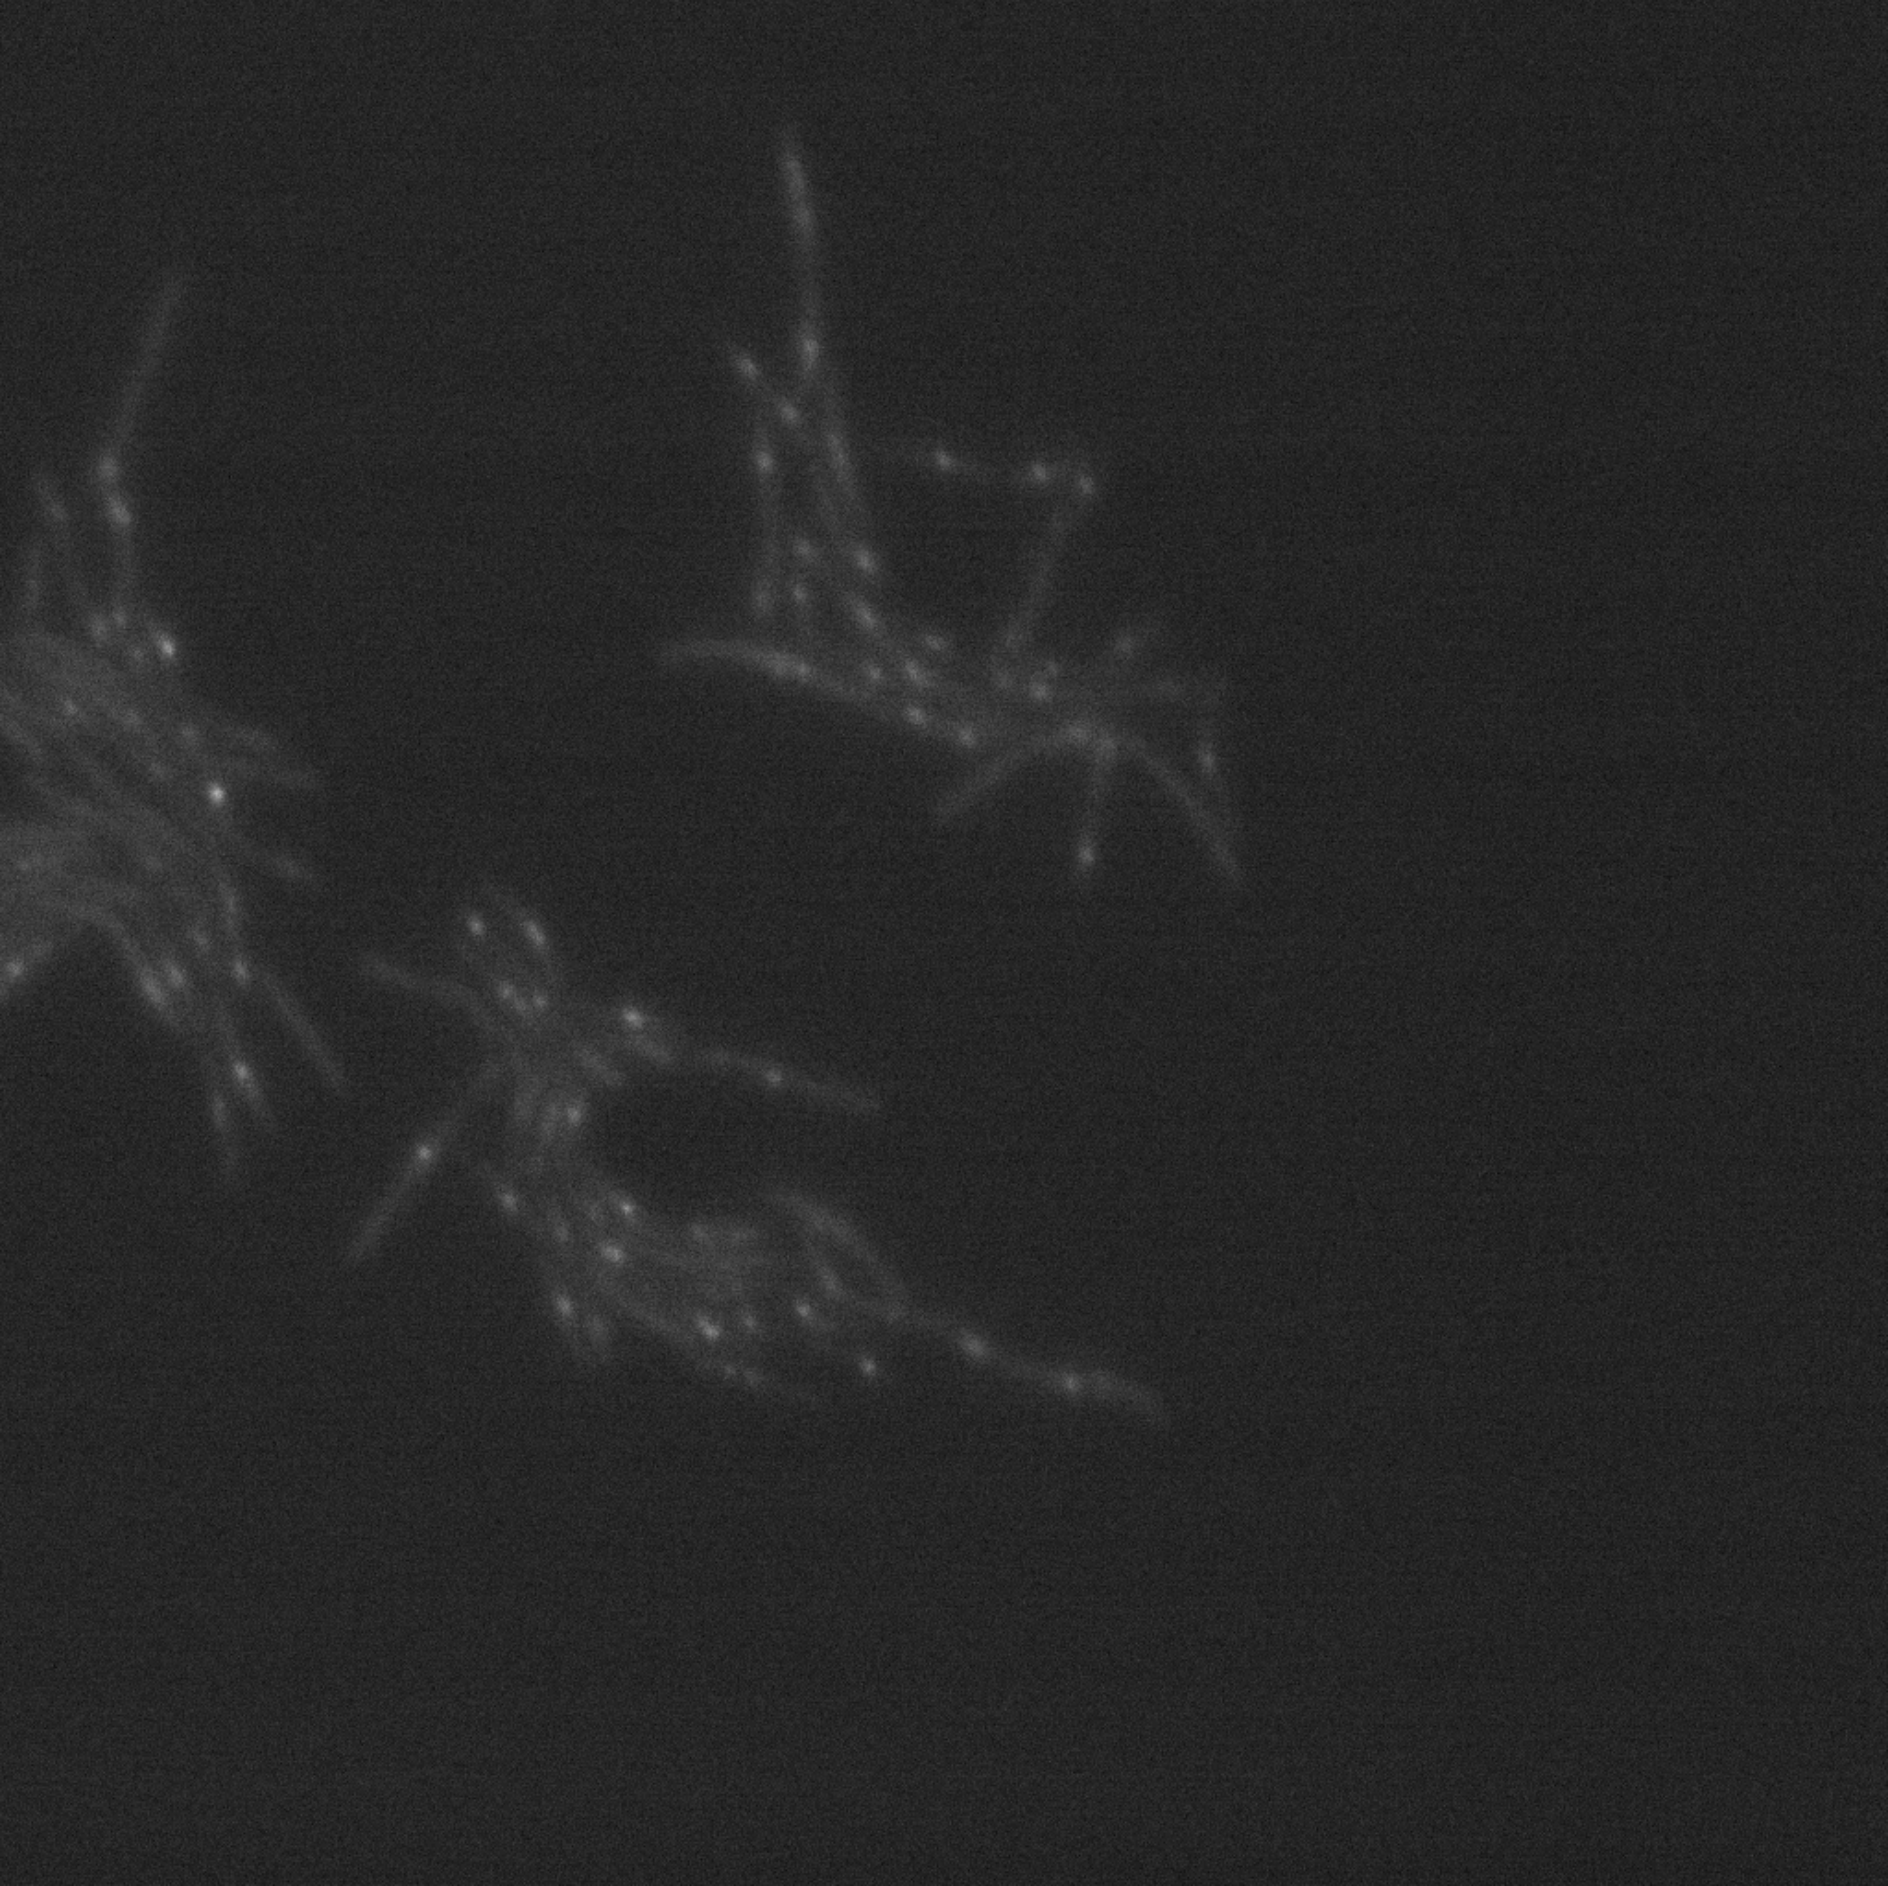
\includegraphics[width=\textwidth]{images/input-channel-1.png}
    \caption{\centering Kanał fluorescencji.}
  \end{subfigure}
  \hfill
  \begin{subfigure}[t]{.45\textwidth}
    \centering
    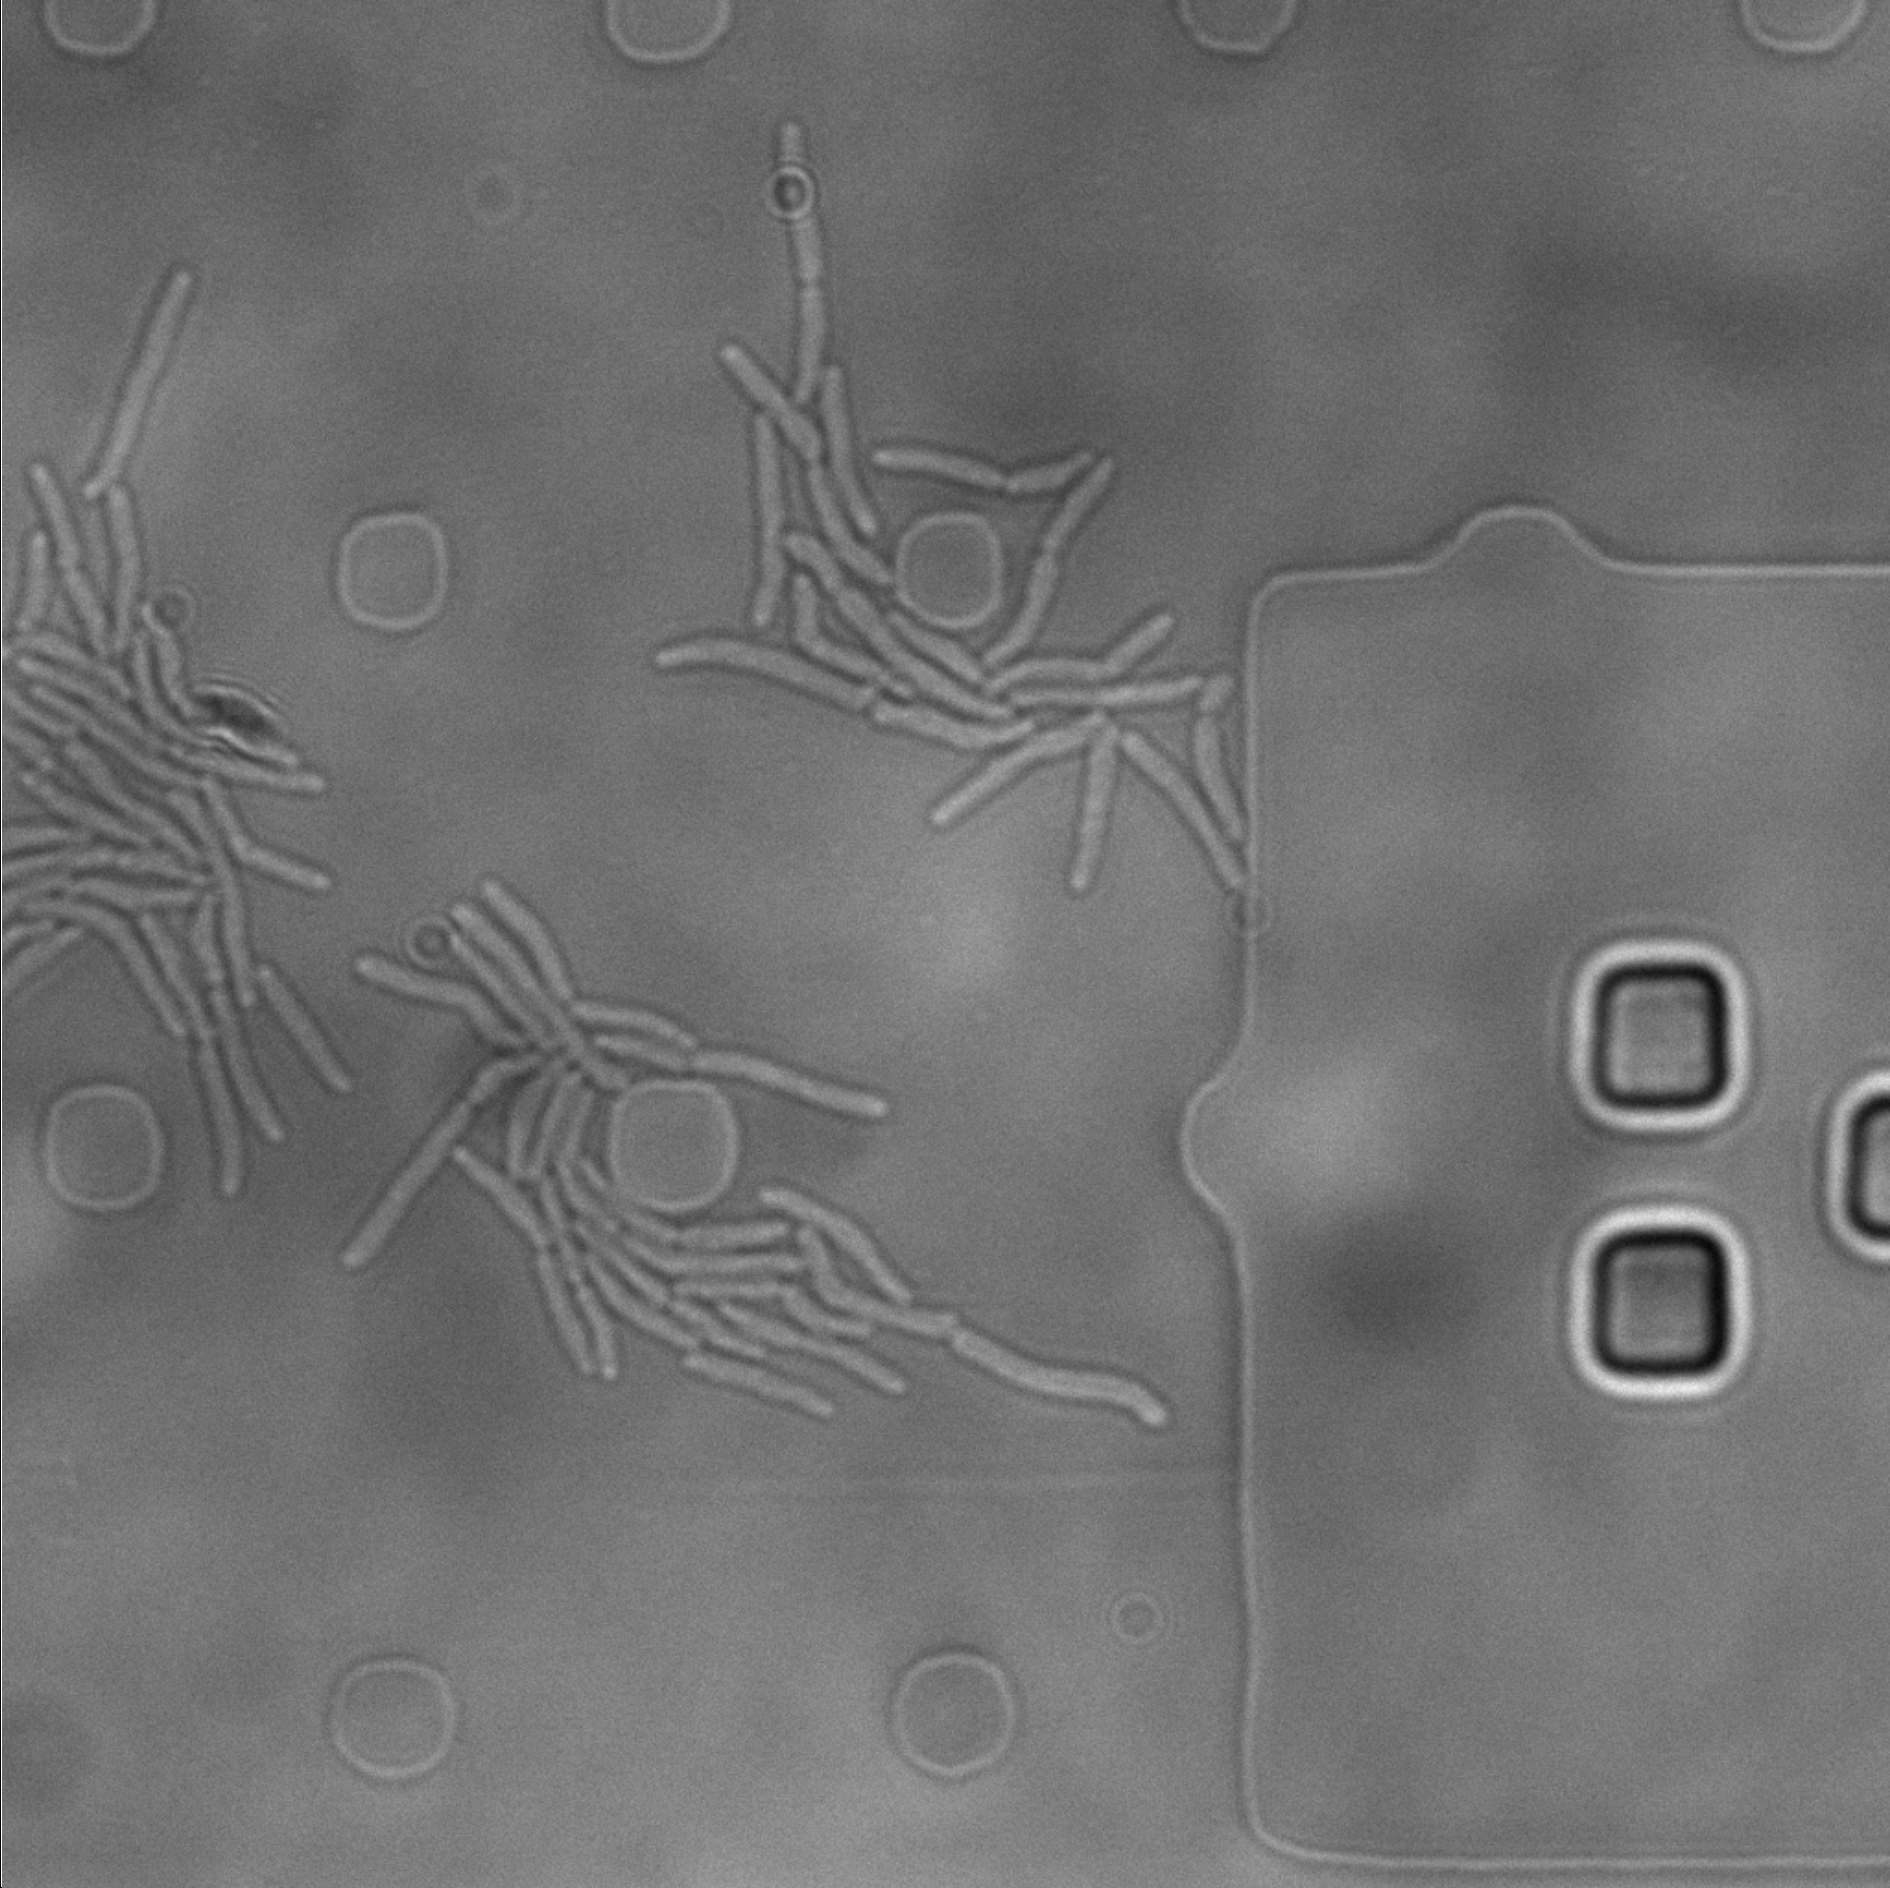
\includegraphics[width=\textwidth]{images/input-channel-2.png}
    \caption{\centering Kanał światła widzialnego w~kontraście DIC.}
  \end{subfigure}
  \hfill

  \caption{Dwa kanały tej samej klatki przykładowego nagrania.}
  \label{fig:input-images}
\end{figure}


\subsection{Pożądany efekt}

Celem pracy, który został opisany dokładniej w~rozdziale \ref{sec:target}, jest uproszczenie części procesu pozyskiwania danych o~cyklu komórkowym prątków z~gatunku \emph{M.~smegmatis}.
Narzędzie stworzone na potrzeby tej pracy ma pomóc badaczom w~żmudnym procesie oznaczania komórek na nagraniach.
Optymistyczny scenariusz zakłada że program, przy niewielkiej interakcji ze strony użytkownika, oznaczy komórki na wszystkich obrazach, zachowując przy tym informacje na temat pochodzenia każdej z~nich.
Oznaczenie komórki oznacza odnalezienie krzywej lub linii łamanej przechodzącej przez środek komórki.
Taki opis komórki pomoże nie tylko przy analizie zmian długości komórek, ale także pozwoli odczytać profil intensywności takiego oznaczenia z~kanału fluorescencji.
Dodatkowym atutem byłaby możliwość edycji tego typu zaznaczeń w~przypadkach gdy program nie wyznaczył ich poprawnie.

Ze względu na słabą jakość nagrań oraz często występujące na obrazach artefakty, automatyczne oznaczanie może nie być możliwe przy niektórych klatkach lub nawet całych nagraniach.
W takich przypadkach użytkownik powinien mieć możliwość ręcznego stworzenia oznaczeń.

\section{Powiązane prace}

Badania biologii prątków z~wykorzystaniem mikroskopii fluorescencyjnej dotyczą przede wszystkim dynamiki replikacji DNA chromosomalnego, segregacji nowo zreplikowanych regionów chromosomu oraz analiz organizacji chromosomu na poziomie pojedynczych komórek\cite{paper:watching-dna-replication}\cite{paper:protein-responsibility}.

W literaturze opisano wiele metod wykrywania prątków na obrazach wykonanych przy pomocy mikroskopu.
W celach diagnostycznych, do identyfikacji chorobotwórczych prątków wykorzystuje się techniki mikroskopii fluorescencyjnej\cite{paper:detection-of-tb-with-ip} oraz metody mikroskopowe nie bazujące na zjawisku fluorescencji\cite{paper:ip-techniques-for-identifying-tb}.
Analiza uzyskanych zdjęć polega najczęściej na dokonaniu segmentacji obrazu na komórki gruźlicy i~pozostałe obszary.
Efekt takiego działania pozwala na stwierdzenie obecności lub nieobecności komórek na obrazie, a~także na określeniu ich zagęszczenia i~lokalizacji.
O ile metody te niewątpliwie są bardzo ważne w~diagnostyce, o~tyle niekoniecznie sprawdzą się w~przypadku analizy danych na poziomie pojedynczych komórek.

%Duża część prac opiera się na analizie kolorów
%Niektóre metody bazują na odpowiednim sposobie przygotowania zdjęć (np. zabarwieniu tła na określony kolor\cite{paper:detection-of-tb-with-ip}).

Podobnym zagadnieniem, niekoniecznie w~kontekście dziedziny, ale z~perspektywy przetwarzania obrazów, jest wykrywanie nicieni.
Jeden z~gatunków, \emph{Caenorhabditis elegans}, od wielu lat jest organizmem modelowym w~badaniach organizmów eukariotycznych\cite{wiki:c-elegans}.
\emph{C.~elegans}, podobnie jak prątki, ma symetryczny pałeczkowaty kształt przypominający robaka.
Badania takich bezkręgowców często polegają na analizie danych na poziomie pojedynczego osobnika.
W literaturze można znaleźć prace opisujące metody automatycznego oznaczania i~opisywania tych nicieni.
Ze względu na dużo większy rozmiar w~porównaniu do komórek bakteryjnych, analizy mikroskopowe \emph{C.~elegans} pozwalają na uzyskanie bardzo dobrej jakości danych.
Lepsza jakość nagrań znacząco ułatwia ich późniejszą obróbkę.
Mimo różnic pomiędzy tymi dziedzinami, praca opisana przez Javiera Fernándeza\cite{paper:worm-detection} była w~pewnym stopniu inspiracją do zaproponowanej przeze mnie metody.


\section{Wykrywanie komórek}
\label{sec:cell-detection}

\subsection{Wstęp}

Problem opisany w~sekcji \ref{sec:problem} zdefiniowany jest dla nagrań spod mikroskopu. Postanowiłem jednak najpierw rozwiązać podobny problem, ale zdefiniowany dla pojedynczego obrazu. Rozwiązanie tego problemu mogłoby z~łatwością zostać uogólnione na stos obrazów (nagranie). W~tym rozdziale opiszę rozwiązanie uproszczonego problemu: oznaczanie komórek widocznych na pojedynczym obrazie. Przez ,,oznaczenie komórki'' mam na myśli odnalezienie łamanej przechodzącej przez środek komórki, a~więc jej szkieletu.

\subsection{Dane wejściowe}
\label{sec:detection-input}

Oznaczenie wszystkich komórek widocznych na obrazie można rozłożyć na dwa osobne problemy:
\begin{enumerate}
  \item Określenie liczby oraz lokalizacji poszczególnych komórek
  \item Odnalezienie kształtu poszczególnych komórek.
\end{enumerate}

W niniejszej pracy zdecydowałem się nie rozwiązywać automatycznie pierwszego problemu.
Zamiast tego użytkownik zobowiązany jest ręcznie zaznaczyć dokładnie jeden punkt wewnątrz każdej komórki widocznej na obrazie.
Wymóg ten dotyczy tylko pierwszej klatki nagrania, co opiszę dokładniej w~dalszej części pracy (\ref{sec:cell-tracking}).

Danymi wejściowymi są zatem dwa kanały obrazu $\image$ oraz zbiór punktów $\mathbf{P}$ lokalizujących komórki.

\subsection{Wybór kanału i~wstępne przetwarzanie obrazu}

Obraz wejściowy składa się z~dwóch podstawowych kanałów (\ref{sec:input-images}).
Chcąc jak najdokładniej oznaczyć początek i~koniec komórki, a~także miejsca ich podziału, postanowiłem wybrać kanał, który zawiera wyraźną informację o~krawędziach w~tych miejscach.
O ile kanał z~fluorescencją mógłby bardzo dobrze sprawdzić się do określenia liczby oraz lokalizacji poszczególnych komórek (w~przypadku ich niewielkiej liczby), o~tyle drugi kanał zawiera dużo dokładniejszą informację na temat krawędzi komórek.

Celem wstępnego przetwarzania obrazu wejściowego jest w~tym przypadku oddzielenie poszczególnych komórek od otoczenia, zachowując przy tym informację na temat ich krawędzi. W~ramach pracy przeprowadziłem wiele testów mających na celu odnalezienie narzędzia spełniającego ten cel. Krawędzie otrzymywane za pomocą filtrów czy algorytmów do ich wyszukiwania często były nieciągłe. Dobierając inne parametry często pojawiały się niechciane zaznaczenia wewnątrz komórek.

Ostatecznie zdecydowałem się użyć narzędzia które nie jest związane z~wykrywaniem krawędzi. Zaobserwowałem, że zdjęcia zrobione tą techniką mają pewne specyficzne właściwości. Komórki są na nich dość równomiernie oświetlone, przez co dobrze widać ich pałeczkowaty kształt. Każdą komórkę otacza też ciemne obramowanie.

\subsubsection{Mapa indeksów kształtu}

Postanowiłem spróbować wyliczyć mapę indeksów kształtu\cite{paper:shape-index} (ang. shape index map) dla obrazu wejściowego, na którym wcześniej zastosowałem rozmycie gaussowskie. Indeks kształtu to liczba z~przedziału $[-1, 1]$ przyporządkowana na podstawie ,,lokalnego kształtu'' powierzchni. Jest to niezmiennicza na skalę (ang. scale invariant) miara, która dzieli powierzchnię na obszary wypukłe, wklęsłe i~hiperboliczne (rysunek \ref{fig:shape-index-range}). Obraz wejściowy interpretowany jest tutaj jako mapa wysokości. Zastosowanie rozmycia gaussowskiego w~pierwszym kroku jest niezbędne w~tym przypadku ze względu na nieodporność tej miary na szum obecny na obrazie wejściowym. Do wyliczenia mapy indeksów skorzystałem z~wtyczki dla programu ImageJ autorstwa Johannesa Schindelina\cite{plugin:shape-index-map}.

\begin{figure}
  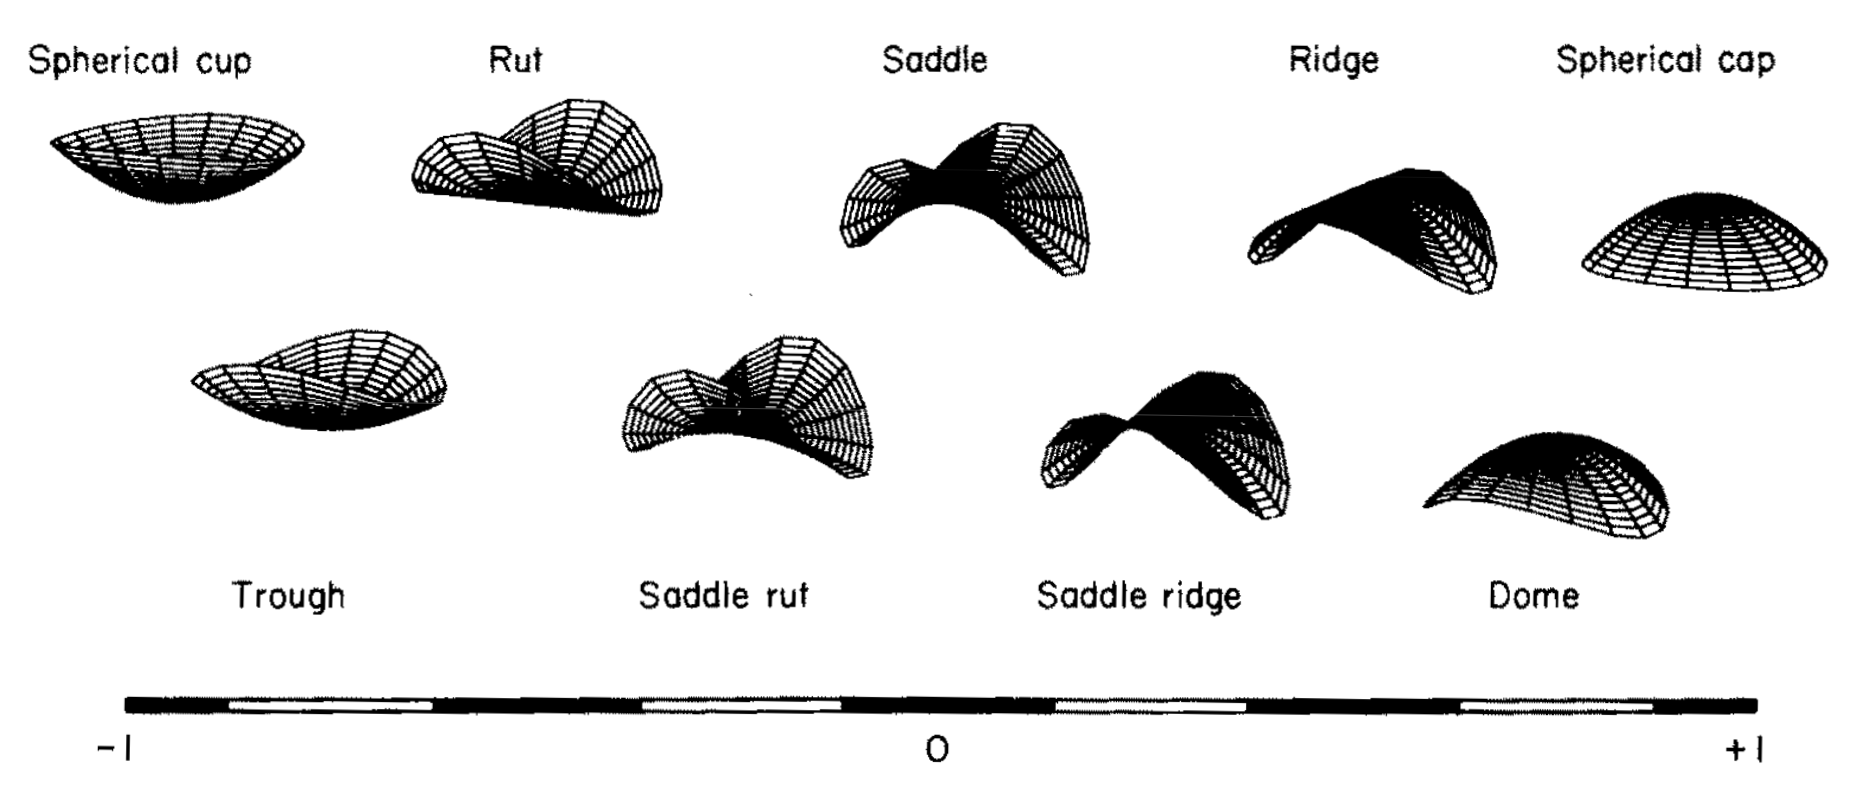
\includegraphics[width=\textwidth]{images/shape-index-range.png}
  \caption{Skala indeksu kształtu z~podziałem na dziewięć kategorii. \cite{paper:shape-index}}
  \label{fig:shape-index-range}
\end{figure}

Okazało się, że na wynikowej mapie otoczenie komórek interpretowane jest jako obszar wklęsły, w~przeciwieństwie do samych komórek, których wnętrze oznaczane jest indeksami kształtów wypukłych.
Własność ta zachodzi dla większości testowych obrazów nawet przy stosunkowo dużym zagęszczeniu komórek.

\subsection{Szkieletyzacja i wstępna detekcja komórek}

Zgodnie z~powyższą obserwacją, możemy łatwo oddzielić komórkę od jej otoczenia na obrazie ustalając pewien próg $t \approx 0$ dla indeksu kształtu.
Załóżmy przez chwilę, że binaryzując w~ten sposób mapę indeksów kształtu otrzymamy obraz $\image_{bin}$, na którym każdy piksel leżący wewnątrz dowolnej komórki będzie miał wartość $1$, natomiast każdy piksel należący do zewnętrznego obrysu dowolnej komórki (nie należący do komórki, lecz sąsiadujący z~pikselem należącym do niej) będzie miał wartość $0$.
Przy takim założeniu każda komórka jest niezależną ,,wyspą'' na binarnym obrazie $\image_{bin}$.
Chcąc odnaleźć łamaną przechodzącą przez środek komórki, chcemy tak naprawdę znaleźć łamaną, która jest równoodległa do jej krawędzi.
Analogiczny problem rozwiązują algorytmy do wyznaczania szkieletu.
Ich celem jest odnalezienie dla danego kształtu zbioru punktów równoodległych do co najmniej dwóch brzegów.

Na potrzeby tej pracy do szkieletyzacji użyta została implementacja algorytmu ,,3D thinning algorithm''\cite{algo:3d-thinning} w~formie pluginu dla programu ImageJ\cite{plugin:skeletonize-3d}.
Mimo to że wtyczka pozwala na szkieletyzację obrazów 3D, w~tym przypadku została użyta do przetworzenia pojedynczego obrazu 2D.
Wynikiem szkieletyzacji jest binarny obraz o~pewnych właściwościach.
Każdy aktywny piksel można przyporządkować do trzech grup:
\begin{itemize}
  \item końcówki -- mają mniej niż 2 sąsiadujące aktywne piksele
  \item węzły -- mają więcej niż 2 sąsiadujące aktywne piksele
  \item połączenia -- mają dokładnie 2 sąsiadujące aktywne piksele.
\end{itemize}
Przedstawiając szkielet jako graf, końcówki tworzyłyby wierzchołki o~stopniu równym $1$ lub $0$, wierzchołki o~większych stopniach przedstawiałyby zbiory sąsiadujących ze sobą węzłów, natomiast krawędzie reprezentowałyby zbiory sąsiadujących ze sobą połączeń (zakończonych zbiorem węzłów lub końcówką). Taką reprezentację grafową można uzyskać za pomocą kolejnej wtyczki dla programu ImageJ tego samego autora\cite{plugin:analyze-skeleton}. Poza standardowymi informacjami wierzchołki i~krawędzie utworzonego za jej pomocą grafu przechowują zbiory pikseli które reprezentują.

Ze względu na specyficzny kształt komórki można zaobserwować następującą właściwość: po przeprowadzeniu szkieletyzacji obrazu $\image_{bin}$, o~ile przyjęte wcześniej założenie jest spełnione, szkielet każdej z~komórek składa się dokładnie z~dwóch końcówek i~połączeń między nimi. Graf opisujący komórkę będzie zawierał w~takim przypadku dokładnie dwa wierzchołki i~jedną krawędź łączącą je ze sobą. Mając do dyspozycji zbiór punktów $\mathbf{P}$ lokalizujących komórki, można teraz w~łatwy sposób odnaleźć dla każdej z~nich graf ją opisujący. Jednym ze sposobów może być wyszukanie dla każdego punktu ze zbioru $\mathbf{P}$ krawędzi która znajduje się najbliżej tego punktu, gdzie odległość między punktem a~krawędzią zdefiniowana jest jako odległość między punktem, a~najbliższym pikselem, który należy do zbioru opisywanego przez tę krawędź.

\subsection{Wybór krawędzi w węzłach}
\label{sec:spine-extending}

Niestety przyjęte założenie o~tym, że każdy piksel należący do zewnętrznego obrysu dowolnej komórki będzie miał wartość $0$, nie zawsze jest spełnione. W~realistycznym scenariuszu zdarza się, że jedna z~końcówek komórki znajduje się na tyle blisko innej komórki, że wstępne przetwarzanie i~progowanie obrazu nie powoduje ich rozdzielenia na obrazie binarnym. Czasem artefakty widoczne na obrazie wejściowym powodują, że wyspa na obrazie binarnym zawiera nie tylko komórkę, ale także fragment innego kształtu. W~zdecydowanej większości takich przypadków szkielet komórki można opisać spójnym podgrafem o~stopniu 2 grafu reprezentującego szkielet wyspy zawierającej komórki.

Wstępna detekcja szkieletu danej komórki polega, tak jak w~scenariuszu optymistycznym, na odnalezieniu krawędzi $\{v_0, u_0\}$ w~grafie $\mathbf{G}$ leżącej najbliżej punktu opisującego komórkę, a~następnie na stworzeniu z~niej i~jej wierzchołków nowego grafu $\mathbf{S}_0$. Tak utworzony szkielet rozszerzany jest później zgodnie z~następującym algorytmem:

\par\bigskip
\begin{algorithmic}
\FORALL{$v \in \{ v_0, u_0 \}$}
  \LOOP
    \STATE
      $\text{E}_v \gets$ zbiór krawędzi $e \in E(\mathbf{G}) - E(\mathbf{S}_n)$ incydentnych do $v$,\newline
      \hphantom{$\text{E}_v \gets$} takich że graf $\mathbf{S}_n + e$ nie posiada cykli
    \IF{$\text{E}_v = \O$}
      \STATE \textbf{break}
    \ENDIF
    \STATE $\{v, u\} \gets \argmax_{e \in \text{E}_v} \ q_v(e)$
    \STATE $\mathbf{S}_{n+1} \gets \mathbf{S}_n + \{v, u\} $
    \STATE $v \gets u$
  \ENDLOOP
\ENDFOR
\end{algorithmic}
\par\bigskip

\noindent
W powyższym algorytmie oznaczenie $E(\mathbf{G})$ opisuje zbiór krawędzi grafu $\mathbf{G}$.
Wyrażenie $\mathbf{S} + e$ oznacza graf utworzony poprzez dodanie do grafu $\mathbf{S}$ krawędzi $e$ oraz jej wierzchołków.
Funkcja $q_v(e)$ jest tutaj funkcją oceny, która służy do wyboru najmocniej związanej krawędzi. Siłą wiązania nazywam najniższą wartość indeksu kształtu (oryginalnego obrazu) dla piksela leżącego na krawędzi $e$, w~okolicy wierzchołka $v$ (w~odległości nie większej niż pewna stała $d$ od środka masy pikseli tworzących węzeł $v$).

Takie rozwiązanie sprawdza się dobrze dla komórek, których szkielet znajduje się w grafie $\mathbf{G}$, oraz jego zakończenia w~tym grafie mają stopień $1$. Pomijam na ten moment przypadek, gdy szukany szkielet komórki nie istnieje w~grafie $\mathbf{G}$. W~pozostałych przypadkach przynajmniej jedno z~zakończeń szukanego podgrafu $\mathbf{S}$ ma w~grafie $\mathbf{G}$ stopień większy niż $1$. Zatem, o~ile funkcja oceny $q_v(e)$ sprawdzi się dobrze jeśli chodzi o~dobór krawędzi należących do szukanego szkieletu komórki, uzyskany na końcu algorytmu graf $\mathbf{S}_n$ będzie nadgrafem szukanego szkieletu $\mathbf{S}$. W~takim przypadku jego ,,nadmiarowa'' część należy do szkieletu innej komórki lub jest wynikiem artefaktu widocznego na oryginalnym obrazie. Drugi przypadek pozostawiam do ręcznego rozwiązania użytkownikowi. Pierwszy natomiast, nachodzące na siebie szkielety komórek, rozwiązuję automatycznie.

\subsection{Rozwiązywanie konfliktów}
\label{sec:fix-conflicts}

Rozdzielanie nachodzących na siebie komórek nazwałem ,,rozwiązywaniem konfliktów''. Niech $\mathbf{\Sigma}_0$ będzie zbiorem wszystkich znalezionych szkieletów komórek, natomiast $X(\mathbf{\Sigma})$ zbiorem par szkieletów nachodzących na siebie, należących do zbioru $\mathbf{\Sigma}$. Rozwiązywanie konfliktów przebiega w~następujący sposób:

\par\bigskip
\begin{algorithmic}

\WHILE{$X(\mathbf{\Sigma}_n) \neq \O$}
  \STATE $\{S_x, S_y\} \gets$ dowolna para ze zbioru $X(\mathbf{\Sigma})$
  \STATE $\{S_x', S_y'\} \gets$ wynik rozwiązania konfliktu pomiędzy $S_x$ i $S_y$
  \STATE $\mathbf{\Sigma}_{n+1} \gets (\mathbf{\Sigma}_n - \{S_x, S_y\}) \cup \{S_x', S_y'\}$
\ENDWHILE

\end{algorithmic}
\par\bigskip

Sposób w~jaki rozwiązywany jest konflikt pomiędzy dwoma szkieletami, zależy od tego w~jaki sposób nachodzą one na siebie. Kluczową rolę odgrywają tutaj także punkty lokalizujące komórki. W~dalszej części pisząc, o~punkcie charakterystycznym komórki, będę miał na myśli punkt leżący na szkielecie będący najbliżej punktu lokalizującego komórkę.

Zaimplementowałem dwie metody rozwiązywania konfliktów, które stosuję w~zależności od rozmieszczenia punktów charakterystycznych.
W obu przypadkach rozwiązanie konfliktu pomiędzy komórkami polega na skróceniu ich w~taki sposób, by nie nachodziły one na siebie.

\subsubsection{Przyłączenie części wspólnej do jednej z komórek}

Po rozwiązaniu konfliktu za pomocą tej metody, jedna z~komórek pozostanie niezmieniona.
Druga zostanie skrócona w~taki sposób, że jej nową końcówką stanie się miejsce, w~którym obie komórki się spotykały.
Rozwiązanie takie stosuje w~dwóch przypadkach:
\begin{enumerate}
  \item Gdy oba punkty charakterystyczne znajdują się poza częścią wspólną, ale po tej samej stronie części wspólnej.
  \item Gdy punkt charakterystyczny pierwszej z~komórek znajduje się wewnątrz części wspólnej, a~drugiej poza nią, oraz pierwsza komórka nie ma żadnej krawędzi poza częścią wspólną, w~kierunku przeciwnym do punktu charakterystycznego drugiej komórki.
\end{enumerate}

W pierwszym przypadku część wspólna przydzielana jest do tego szkieletu z~którym jest mocniej związana (siłę wiązania określam w~podobny sposób jak w~opisanym wcześniej algorytmie konstrukcji szkieletu).
W drugim przypadku sprawa jest prosta -- część wspólna zostaje przydzielona do szkieletu którego punkt charakterystyczny leży w~części wspólnej.

\begin{figure}[H]
  \centering
  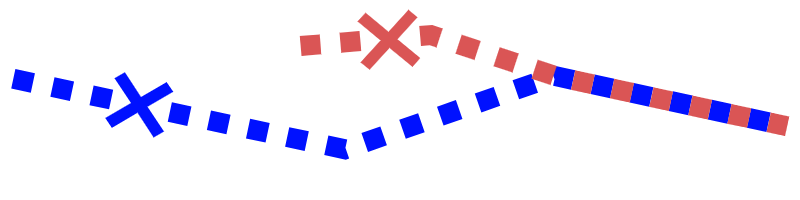
\includegraphics[valign=m,width=0.35\textwidth]{images/overlap-out-out-assign.png}
  $\rightarrow$
  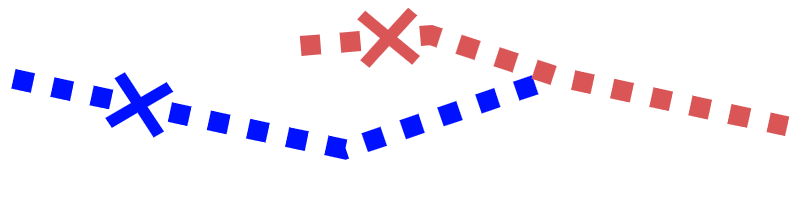
\includegraphics[valign=m,width=0.35\textwidth]{images/overlap-out-out-assign-solved.png}
\end{figure}

\begin{figure}[H]
  \centering
  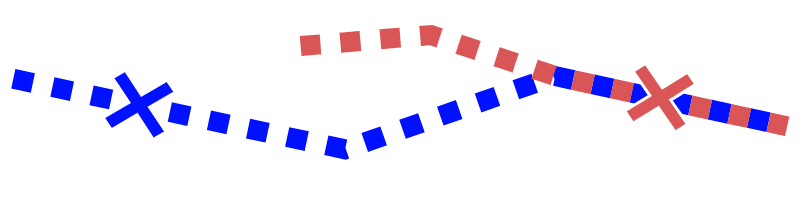
\includegraphics[valign=m,width=0.35\textwidth]{images/overlap-out-in-assign.png}
  $\rightarrow$
  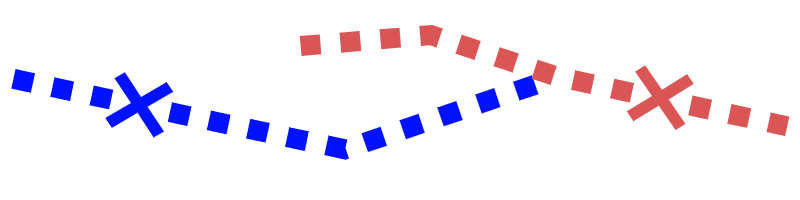
\includegraphics[valign=m,width=0.35\textwidth]{images/overlap-out-in-assign-solved.png}
\end{figure}

% rysunki mogłyby być bezpośrednio pod punktami
% można by dodać jeszcze legendę jak wygląda komórka, punkt charakterystyczny, część wspólna

\subsubsection{Podzielenie części wspólnej}

We wszystkich pozostałych przypadkach stosuję drugą metodę, polegającą na skróceniu obu komórek.
Rozwiązanie konfliktu polega tutaj na znalezieniu najsłabszego punktu (mającego najniższy indeks kształtu) leżącego w~części wspólnej pomiędzy punktami charakterystycznymi, a~następnie odpowiednim skróceniu obu szkieletów do tego punktu.

\begin{figure}[H]
  \centering
  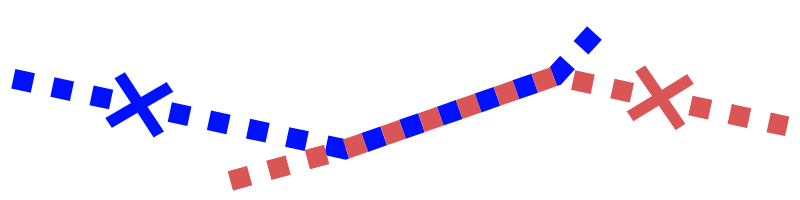
\includegraphics[valign=m,width=0.35\textwidth]{images/overlap-out-out-split.png}
  $\rightarrow$
  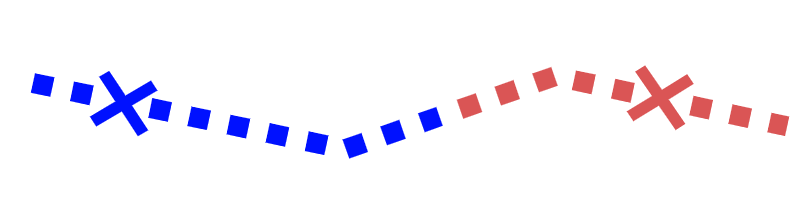
\includegraphics[valign=m,width=0.35\textwidth]{images/overlap-out-out-split-solved.png}
\end{figure}

\begin{figure}[H]
  \centering
  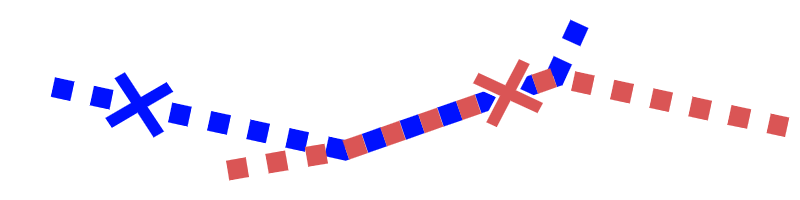
\includegraphics[valign=m,width=0.35\textwidth]{images/overlap-out-in-split.png}
  $\rightarrow$
  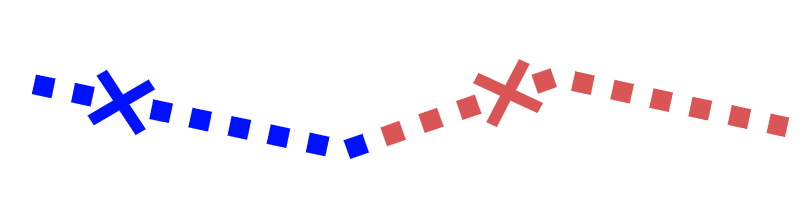
\includegraphics[valign=m,width=0.35\textwidth]{images/overlap-out-in-split-solved.png}
\end{figure}

\begin{figure}[H]
  \centering
  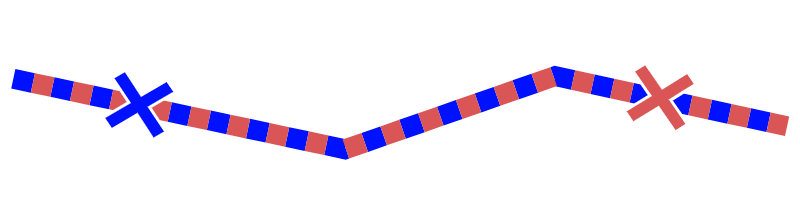
\includegraphics[valign=m,width=0.35\textwidth]{images/overlap-in-in-split.png}
  $\rightarrow$
  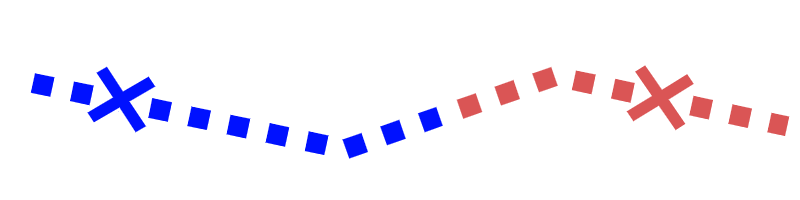
\includegraphics[valign=m,width=0.35\textwidth]{images/overlap-in-in-split-solved.png}
\end{figure}

\subsubsection{Nakładanie się wielokrotne}

Dwa szkielety mogą mieć więcej niż jeden konflikt równocześnie.
Taka sytuacja nie zdarza się często, ale jest prawdopodobna.
W tym przypadku w~każdej iteracji rozwiązywany jest jeden z~takich konfliktów za pomocą sposobów opisanych powyżej.

\begin{figure}[H]
  \centering
  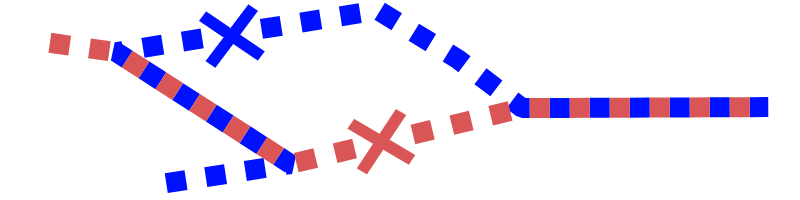
\includegraphics[valign=m,width=0.3\textwidth]{images/overlap-multi.png}
  $\rightarrow$
  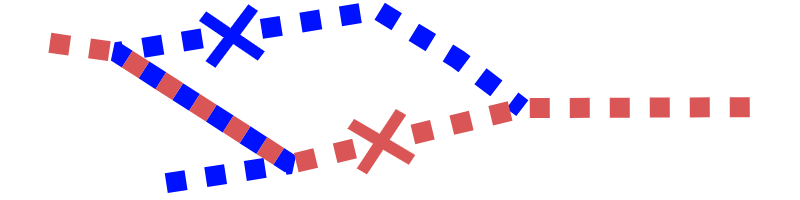
\includegraphics[valign=m,width=0.3\textwidth]{images/overlap-multi-solved1.png}
  $\rightarrow$
  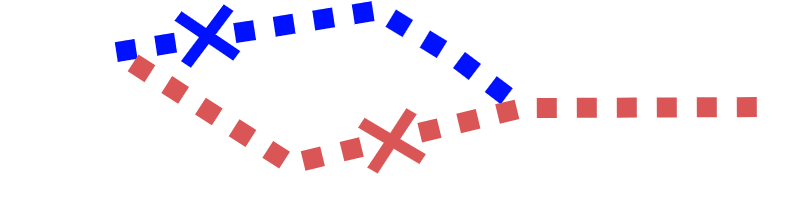
\includegraphics[valign=m,width=0.3\textwidth]{images/overlap-multi-solved2.png}
\end{figure}

\subsection{Uzyskiwanie linii łamanej}

Po rozwiązaniu wszystkich konfliktów każdy szkielet opisuje pewną komórkę.
Kolejnym krokiem jest konwersja reprezentacji grafowej (która zawiera zbiór pikseli opisujących szkielet) do linii łamanaj.
W takiej formie użytkownik będzie mógł ręcznie modyfikować zaznaczenia komórek korzystając ze standardowego interfejsu programu ImageJ.
Pierwsza wersja linii łamanej powstaje ze wszystkich punktów tworzących krawędzie i~końcówki szkieletu, a~także ze środków masy jego węzłów.
Następnie geometria łamanej jest upraszczana za pomocą algorytmu Ramera--Douglasa--Peuckera\cite{algo:ramer}\cite{algo:douglas-peucker}.
Algorytm ten eliminuje punkty, których usunięcie nie wpływa znacząco na kształt łamanej tj. po ich usunięciu odległość uproszczonej łamanej od oryginalnej jest nie większa niż pewna przyjęta stała.

\subsection{Korekta końcówek}
\label{sec:correct-endpoints}

Ostatnim krokiem oznaczania komórek jest korekta końcówek.
Potrzeba korekty wynika z~algorytmu szkieletyzacji.
Proces ten polega na erodowaniu binarnego obrazu --- z~tego powodu końcówki szkieletu komórki często oddalone są od faktycznej krawędzi na oryginalnym obrazie.
Dotyczy to tylko zakończeń które reprezentowane są przez wierzchołki mające w~oryginalnym szkielecie obrazu stopień równy $1$.
Nie dzieje się tak w~przypadku, gdy binarny obraz komórki łączy się w~tym miejscu z~inną komórką, a~zakończenie powstało na skutek rozwiązania konfliktu.

Właściwej lokalizacji zakończenia komórki szukam na półprostej tworzonej przez ostatni odcinek łamanej, która ją opisuje.
Mając do dyspozycji obraz binarny na podstawie którego powstał szkielet, szukam zakończenia wyspy leżącego najbliżej początku półprostej.
Jeśli punkt ten leży nie dalej niż pewna przyjęta stała, staje się on nowym zakończeniem łamanej.
Stała którą przyjąłem była nie większa niż przewidywana szerokość komórki.

Proces ten powtarzany jest dla każdego zakończenia komórki wymagającego poprawienia.

\section{Śledzenie komórek w czasie}
\label{sec:cell-tracking}

Do tej pory opisywałem sposób na wykrywanie i~oznaczanie komórek na pojedynczym obrazie, mając do dyspozycji punkty lokalizujące komórki wprowadzone przez użytkownika.
Oryginalny problem dotyczył jednak stosu obrazów przedstawiającego cykl komórkowy bakterii w~czasie.
Uogólnienie opisanego sposobu polega na automatycznym wyznaczaniu dla każdej komórki kilku potencjalnych punktów ją lokalizujących, na podstawie łamanej opisującej tę komórkę w~poprzedniej klatce nagrania naniesionej na aktualną klatkę.
Następnie wybierane są te punkty (i~stworzone przez nie szkielety), które dały najlepsze efekty względem pewnej funkcji oceny.

Jeśli nowy szkielet komórki jest znacząco krótszy niż łamana opisująca ją na poprzednim obrazie, prawdopodobnie oznacza to, że nastąpił podział komórki. W~takim przypadku wyszukiwany jest kolejny szkielet. Tym razem kandydatów na punkty lokalizujące poszukuję tylko po jednej stronie łamanej. Jeśli pierwszy szkielet powstał na podstawie punktu leżącego bliżej końca łamanej, jego bliźniaczy szkielet prawdopodobnie znajduje się bliżej jej początku i~vice versa.

Po odnalezieniu wszystkich nowych szkieletów zgodnie z~powyższą procedurą, następuje etap rozwiązywania konfliktów, konwersji na linie łamane i~ostatecznej korekty końcówek, tak jak to zostało opisane (\ref{sec:fix-conflicts}--\ref{sec:correct-endpoints}).


Niech $\mathbf{C}_n$ będzie zbiorem łamanych opisujących komórki na $n$-tym obrazie stosu.
Niech $\phi_\sigma(d)$ będzie funkcją która liczbą z~przedziału $[0, 1]$ przyporządkowuje punkty leżące na łamanej $\sigma$, proporcjonalnie do odległości od jej początku (przyjmijmy, że linia łamana ma zdefiniowany ,,kierunek'', tzn. ma początek i~koniec). Niech $S_n(p)$ będzie szkieletem komórki wyznaczonym zgodnie z~metodą opisaną wcześniej (\ref{sec:detection-input}--\ref{sec:spine-extending}) dla punktu lokalizującego $p$ i~$n$-tej klatki nagrania.
Cały proces można zobrazować następującym algorytmem:

\par\medskip
\begin{algorithmic}

\FORALL{$n \in \{ 0, 1, \ldots, n-1 \}$}
  \STATE $\mathbf{\Sigma}_{n+1} \gets \O$
  \FORALL{$\sigma \in \mathbf{C}_n$}
    \STATE $\Sigma \gets \{ S_{n+1}(\phi_\sigma(d)) \ | \ d \in \text{D} \}$
    \STATE $S \gets \argmax_{S \in \Sigma} \ q_\sigma(S)$
    \STATE $\mathbf{\Sigma}_{n+1} \gets \mathbf{\Sigma}_{n+1} \cup \{ S \}$

    \IF{$| S | < 0.9 \cdot | \sigma |$}
      \STATE $\Sigma' \gets \{ S_{n+1}(\phi_\sigma(d')) \ | \ d' \in \text{D}' \}$
      \STATE $S' \gets \argmax_{S' \in \Sigma} \ q_\sigma(S')$
      \STATE $\mathbf{\Sigma}_{n+1} \gets \mathbf{\Sigma}_{n+1} \cup \{ S' \}$
    \ENDIF
  \ENDFOR
  \STATE $\mathbf{\hat{\Sigma}}_{n+1} \gets$ wynik rozwiązania konfliktów w zbiorze $\mathbf{\Sigma}_{n+1}$
  \STATE $\mathbf{C}_{n+1} \gets$ wynik konwersji na łamane i korekty końcówek elementów zbioru $\mathbf{\hat{\Sigma}}_{n+1}$
\ENDFOR

\end{algorithmic}

\noindent
W algorytmie pojawia się zbiór $D \subseteq [0, 1]$ którego elementy dobrałem empirycznie jako $\{ 0.2, 0.4, 0.6, 0.8 \}$.
Zbiór $D' \subset D$ to zbiór, który zależy od wcześniejszego wyboru najlepszego kandydata na szkielet komórki.
Jeśli w~danej iteracji szkielet $S$ powstał na podstawie punktu lokalizującego leżącego na pierwszej połowie łamanej, będzie to zbiór $\{ d \in D \ | \ d > 0.5 \}$ w~przeciwnym wypadku będzie to pozostała część zbioru $D$.

Funkcja $q_\sigma(S)$ jest funkcją oceny szkieletu względem krzywej $\sigma$. Bazuje ona na założeniu, że komórka w~nowej klatce nie powinna zbytnio oddalić się od miejsca w~którym znajdowała się poprzednio.
Dla wszystkich potencjalnych punktów lokalizujących komórkę, wyliczana jest ich odległość od nowo utworzonego szkieletu $S$. Wartość oceny jest odwrotnie proporcjonalna do sumy tych odległości.

\section{Interakcja ze strony użytkownika}

Niestety powyższe działania nie sprawdzą się dobrze w~każdym przypadku.
Jest wiele czynników które utrudniają poprawną detekcję komórek.
Większość z~nich związana jest ze słabą jakością nagrań.
Obrazy są mocno zaszumione, często występują na nich artefakty, czasem płytka na której poruszają się komórki minimalnie się przesuwa, a~innym razem mikroskop traci ostrość na kilka klatek nagrania.
Zapewne można próbować rozwiązać te problemy automatycznie, ale na pewno pojawią się nowe, nie rozważane wcześniej przypadki.
Właśnie z~tego powodu postanowiłem zapewnić użytkownikowi możliwość interaktywnego poprawiania automatycznie stworzonych oznaczeń komórek, ale także całkowicie manualne kontynuowanie detekcji, zachowując przy tym informacje o~historii komórek.

Komórki przedstawione są w~oknie programu jako standardowe zaznaczenia programu ImageJ i~można je edytować za pomocą standardowego interfejsu.
Ponadto stworzyłem dwa dodatkowe narzędzia dla użytkownika.
Pierwsze z~nich służy do rozcinania komórek w~miejscach, w~których się one dzielą.
Mimo że algorytm śledzenia ma mechanizm odpowiedzialny za zauważenie takich zmian, zdarza się że dzieje się to zbyt późno (komórki jeszcze przez pewien czas po podziale znajdują się bardzo blisko siebie).

Drugie narzędzie służy do skracania końcówek zaznaczeń.
Zauważyłem, że częstym problemem jest to, że zaznaczenie wybiega poza krawędzie komórki.
Najczęściej dzieje się to ze względu na występujące na obrazie artefakty lub punkty stałe na płytkach znajdujące się blisko zakończeń komórek.
Żeby przyspieszyć proces poprawiania takich zaznaczeń można skorzystać z~narzędzia do skracania końcówek, które działa podobnie do ,,gumki'' w~popularnych programach graficznych.

Chcąc ręcznie oznaczyć komórki w~kolejnej klatce (zamiast wyliczać je automatycznie na podstawie poprzedniej), użytkownik może skorzystać z~opcji duplikowania klatki. Dzięki temu w~aktualnej klatce pojawią się wszystkie zaznaczenia z~klatki poprzedniej, które następnie można ręcznie dopasować do ich nowej pozycji.


%%%%%%%%%%%%%%%%%%%%%%%%%%%%%%%%%%%%%%%%%%%%%%%%%%%%%%%%%%%%%%%%%%%%%%%%%%%%%%%%%%%%%%%%%%%

\chapter{Opis implementacji}

%%%%%%%%%%%%%%%%%%%%%%%%%%%%%%%%%%%%%%%%%%%%%%%%%%%%%%%%%%%%%%%%%%%%%%%%%%%%%%%%%%%%%%%%%%%


\section{Kod źródłowy}

Kod źródłowy projektu zamieszczony został w~publicznie dostępnym repozytorium w~serwisie GitHub na licencji MIT.
Repozytorium można znaleźć pod adresem
\linebreak\url{https://github.com/rossinek/cell-detector-imagej-plugin}.

Program zaimplementowany jest jako wtyczka do programu ImageJ, napisana w~języku Java. Do automatyzacji procesu budowy wykorzystany został Apache Maven. Wszystkie zależności zostały uwzględnione w~pliku konfiguracyjnym dla Mavena, który odpowiada również za ich pobranie.

Plugin był rozwijany głównie na systemie macOS Catalina, ale został również przetestowany na systemie Windows 10.

\section{Kompilacja i uruchomienie}

Przed zbudowaniem pluginu z~kodu źródłowego należy upewnić się, że zainstalowane są wymagane zależności. Poniższa instrukcja zakłada, że system wyposażony jest w:

\begin{itemize}
  \item Apache Maven w~wersji większej lub równej \texttt{3.3.9}
  \item Java w~wersji 8.
\end{itemize}

Aby zbudować projekt należy skorzystać z~komendy \texttt{mvn}, która spowoduje pobranie wszystkich zależności,  kompilację kodu źródłowego i~wywołanie testów automatycznych.

Zbudowany plugin dla programu ImageJ można znaleźć w~folderze \texttt{target} pod nazwą \texttt{Mtbt\_Plugin-\{wersja\}.jar}. Tak spakowany plugin można zainstalować w~programie ImageJ (lub Fiji) wklejając go do folderu \texttt{jars} w~miejscu gdzie zainstalowany jest program.

Aby uruchomić plugin w~ramach własnej niezależnej instancji ImageJ, po zbudowaniu projektu można uruchomić główną metodę programu komendą
\linebreak\texttt{mvn exec:java -Dexec.mainClass="dev.mtbt.Main"}.


\section{Obsługa pluginu}
\label{sec:user-manual}

Po zainstalowaniu pluginu w~programie ImageJ pojawi się nowe menu \texttt{Mycobacterium} (rysunek \ref{fig:ui-menu}) w~którym znajdują się narzędzia zaimplementowane na potrzeby tej pracy. Poza głównym pluginem (\texttt{Cell detector}) znajdują się tam jeszcze dodatkowe wtyczki służące do importu oraz eksportu komórek, a~także narzędzia pomocne w~rozwoju programu.
\begin{figure}
  \centering
  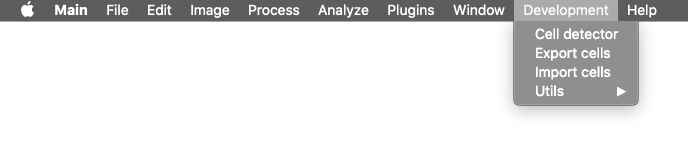
\includegraphics[width=0.7\textwidth]{images/ui-menu.png}
  \caption{Menu programu ImageJ rozszerzone o~wtyczki zaimplementowane na potrzeby tej pracy.}
  \label{fig:ui-menu}
\end{figure}
Główny plugin podzielony jest na trzy kroki:


\begin{enumerate}
  \item Lokalizacja i~wstępna detekcja komórek
  \item Śledzenie komórek w~czasie
  \item Analiza danych
\end{enumerate}

Przed uruchomieniem pluginu należy otworzyć nagranie które chcemy analizować. Po jego uruchomieniu zobaczymy okno pluginu przedstawiające pierwszy krok.
Interfejs pluginu na każdym etapie składa się z~kilku stałych i~kilku zmiennych (w~zależności od aktualnego kroku) części składowych.
Po prawej stronie znajduje się zawartość standardowego okna wielokanałowego stosu obrazów ImageJ.
Dwa suwaki w~dolnej części służą do wyboru kanału oraz klatki nagrania.
Wybór kanału ma wpływ na to, na którym z~nich odbywa się detekcja.
Pierwszym wyborem powinien być kanał przedstawiający komórki oświetlone światłem widzialnym.
Obok suwaka do wyboru klatki znajduje się przycisk start/stop służący do odtwarzania nagrania.
W górnej części panelu znajdującego się po lewej stronie znajdują się kontrolki specyficzne dla danego kroku pluginu. W~jego dolnej części znajdują się narzędzia przydatne na każdym etapie działania pluginu, a~także przyciski do zmiany kroku.


\subsection{Lokalizacja i wstępna detekcja komórek}

Pierwszy etap polega na zaznaczeniu przez użytkownika punktów lokalizujących komórki, a~następnie uruchomieniu wstępnej detekcji (rysunek \ref{fig:ui-step-detector}).
W tym celu należy wcisnąć przycisk \texttt{Select cells}, zaznaczyć każdą komórkę widoczną na pierwszej klatce nagrania klikając w~nią kursorem, a~następnie wcisnąć przycisk \texttt{Run detection}.
W celu poprawienia wstępnej selekcji można skorzystać z~przycisku \texttt{Reset}, który usuwa cały uzyskany do tej pory efekt.

\begin{figure}
  \centering
  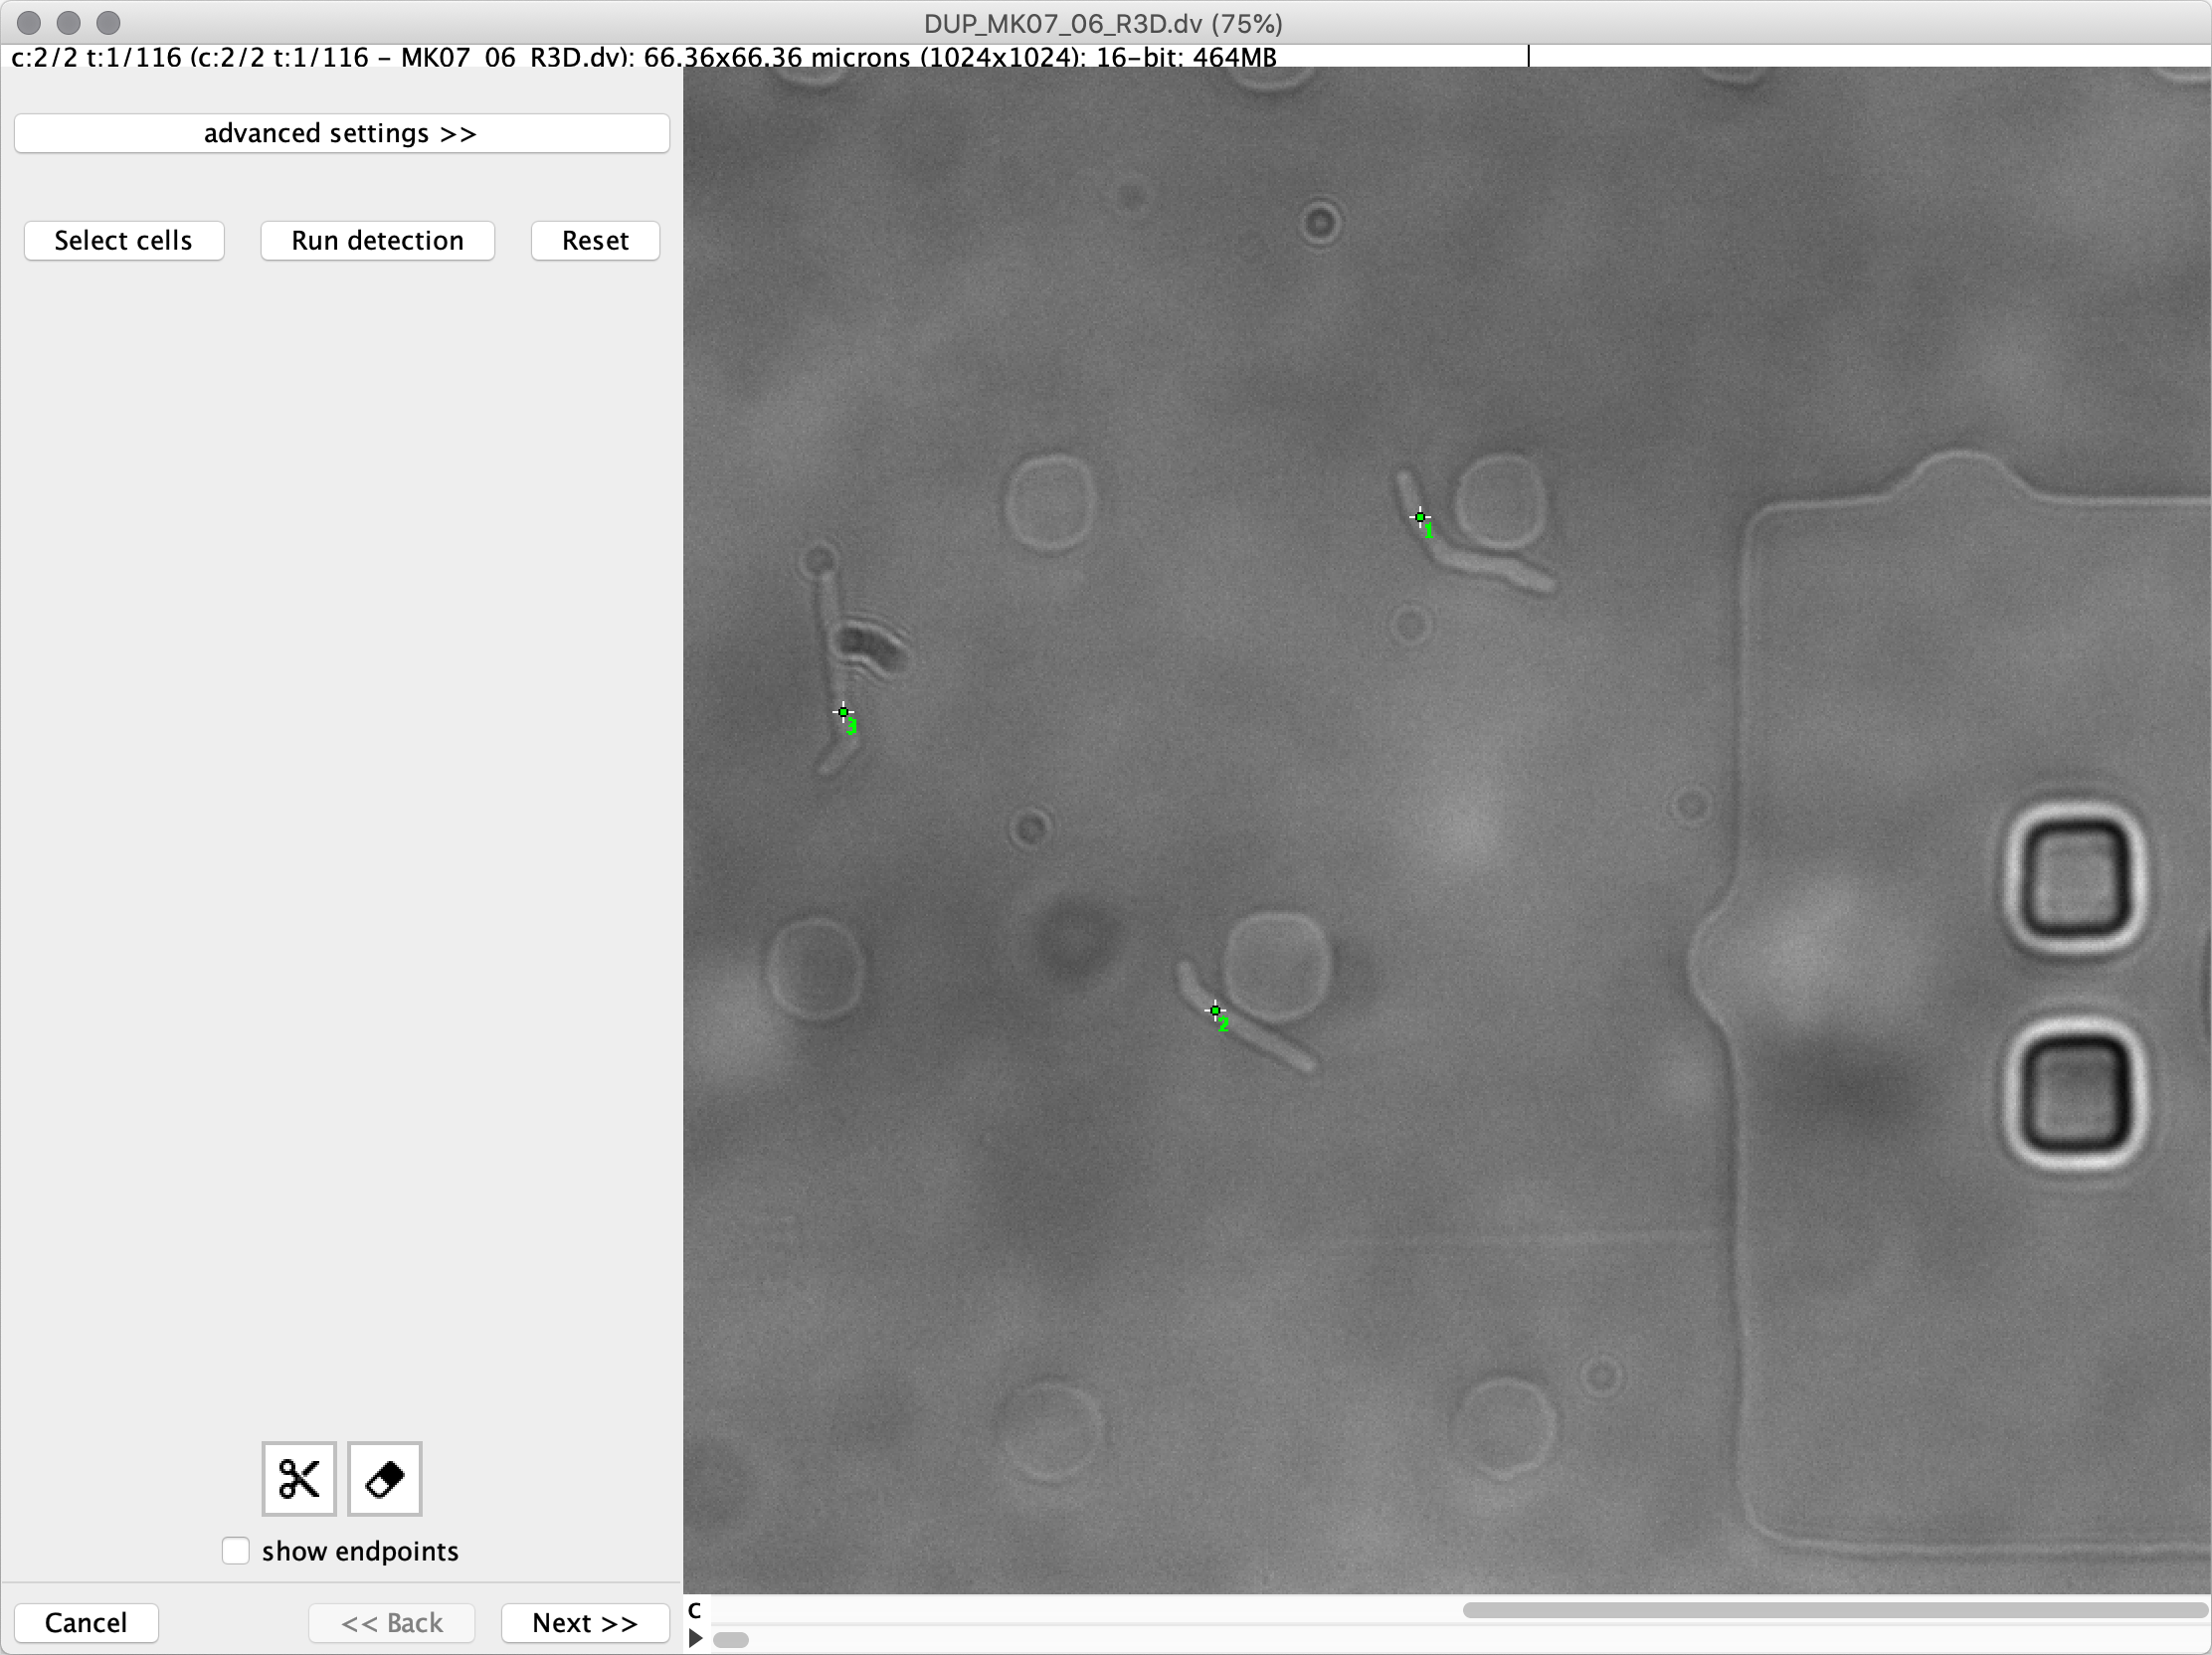
\includegraphics[width=\textwidth]{images/ui-step-detector.png}
  \caption{Pierwszy krok pluginu służący do wstępnej detekcji komórek.}
  \label{fig:ui-step-detector}
\end{figure}

W dodatkowym panelu \texttt{advanced settings} ukryte zostały dodatkowe parametry sterujące procesem detekcji komórek (\ref{sec:cell-detection}), takie jak siła rozmycia gaussowskiego czy wartość progowa użyte na etapie wstępnego przetwarzania obrazu.
Można tam również włączyć podgląd mapy indeksów kształtu, a~także szkieletu na podstawie których przebiega proces detekcji.

\subsection{Śledzenie komórek w czasie}

Kolejnym krokiem jest śledzenie komórek w~czasie (rysunek \ref{fig:ui-step-tracker}).
Użytkownik na tym etapie może zdecydować w~jaki sposób chce dalej pracować.
Może skorzystać z~opcji automatycznego wyliczenia jednej bądź kilku kolejnych klatek (przycisk \texttt{calculate next}) lub zduplikować aktualnie zaznaczone komórki do kolejnej klatki, a~następnie skorzystać z~dostępnych narzędzi i~manualnie je dostosować (\texttt{duplicate}).
Cofając się w~historii do poprzednich klatek można poprawiać zaznaczenia. Można też powtórnie wyliczyć zaznaczenia na danym obrazie, jednak należy wtedy pamiętać, że zaznaczenia w~kolejnych klatkach zostaną usunięte.

\begin{figure}
  \centering
  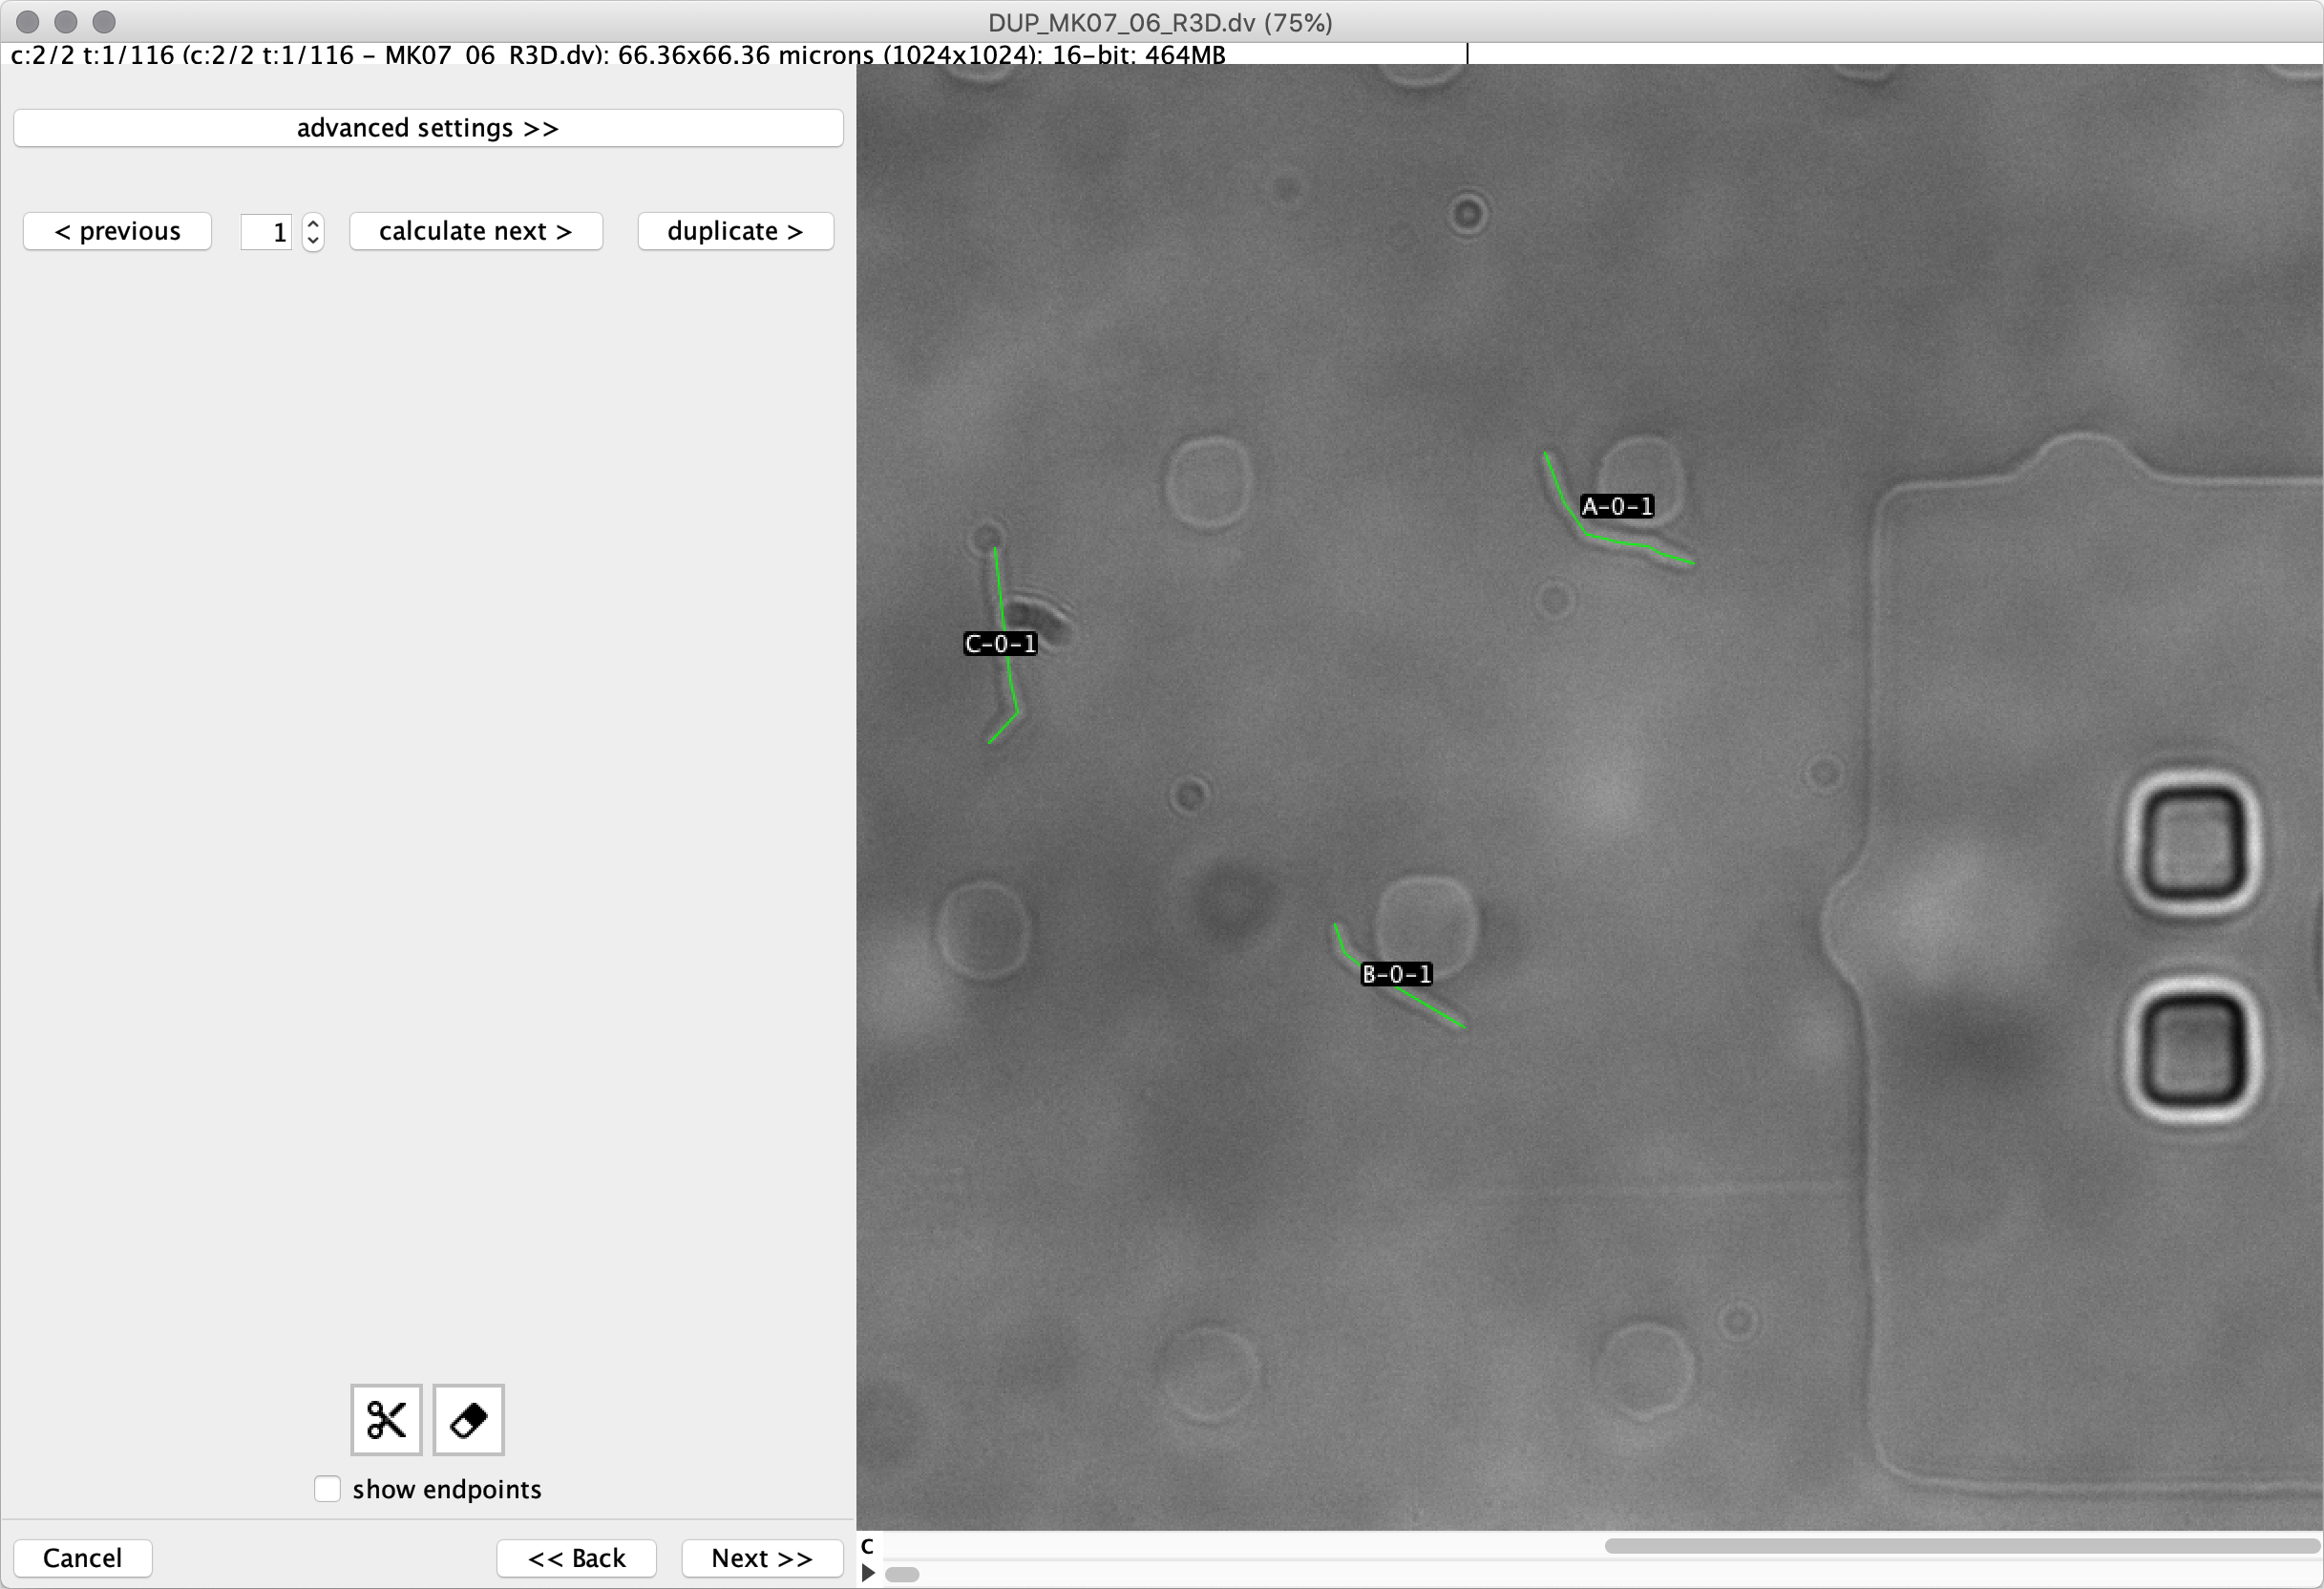
\includegraphics[width=\textwidth]{images/ui-step-tracker.png}
  \caption{Drugi krok pluginu służący do wstępnej śledzenia komórek w~czasie.}
  \label{fig:ui-step-tracker}
\end{figure}

\subsection{Analiza danych}

\begin{figure}
  \centering
  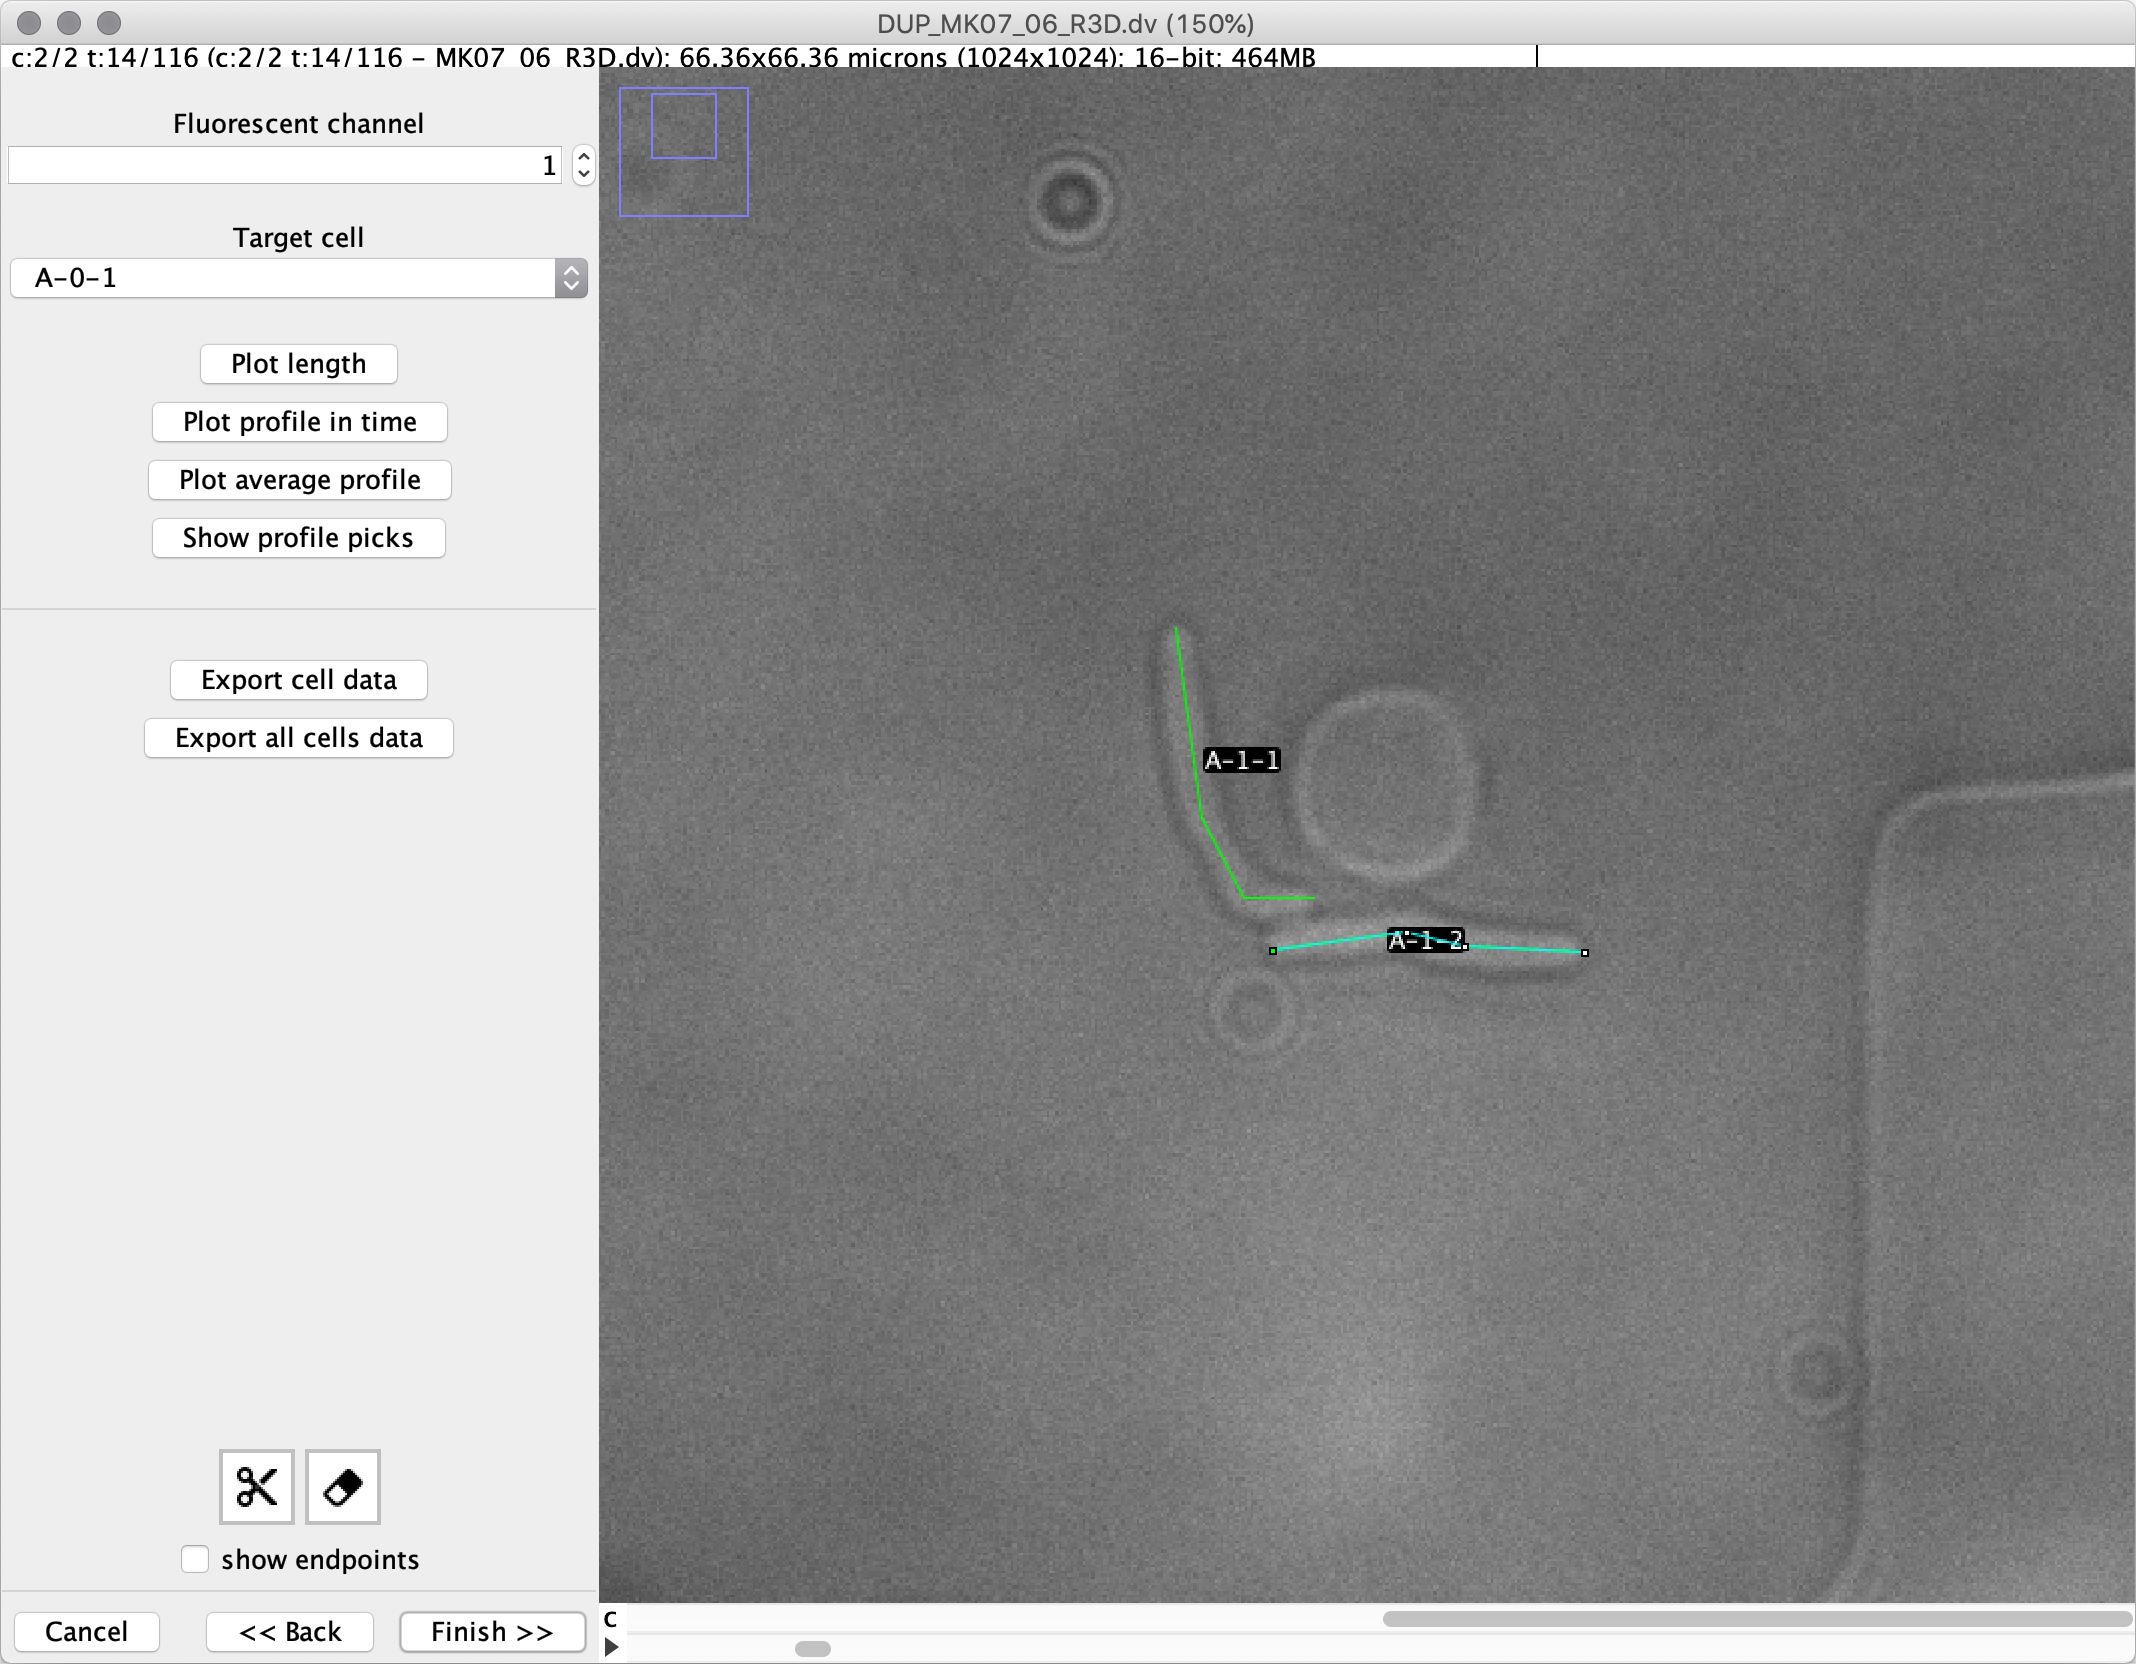
\includegraphics[width=\textwidth]{images/ui-step-measurements.png}
  \caption{Trzeci krok pluginu służący do analizy zaznaczonych komórek.}
  \label{fig:ui-step-measurements}
\end{figure}

Ostatni krok umożliwia analizę danych wyliczonych na podstawie zaznaczonych komórek (rysunek \ref{fig:ui-step-measurements}).
W celu zapewnienia poprawności danych należy najpierw wskazać numer kanału z~fluorescencją. Kolejnym krokiem jest wybór komórki do analizy.
Umieszczona niżej sekcja przycisków pozwala na wyświetlenie kilku rodzajów wykresów (rysunek \ref{fig:ui-plots}):

\begin{itemize}
  \item wykresu przedstawiającego zmianę długości komórki w~czasie
  \item stosu profili intensywności pod łamaną opisującą komórkę na kanale z~fluorescencją (dla każdej klatki w~cyklu komórkowym dla analizowanej komórki)
  \item średniego profilu intensywności pod łamaną opisującą komórkę na kanale z~fluorescencją (przed uśrednieniem oś~X~każdego profilu jest normalizowana do przedziału $[0, 1]$)
  \item umiejscowienia ,,skupisk'' na kanale z~fluorescencją w~czasie.
\end{itemize}

\begin{figure}
  \centering

  \begin{subfigure}[t]{.45\textwidth}
    \centering
    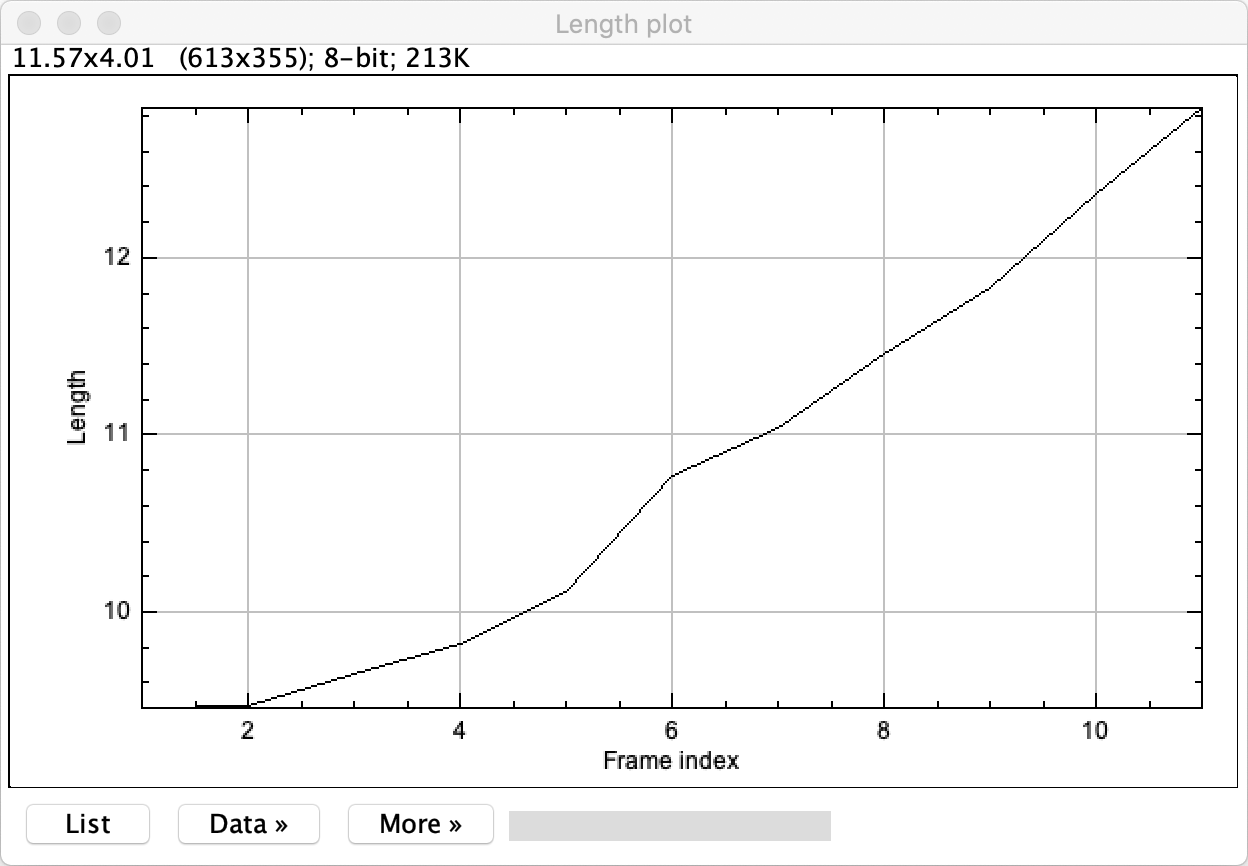
\includegraphics[width=\textwidth]{images/ui-plot-lengths.png}
    \caption{\centering Wykres przedstawiający zmianę długości komórki w~czasie.}
  \end{subfigure}
  \hfill
  \begin{subfigure}[t]{.45\textwidth}
    \centering
    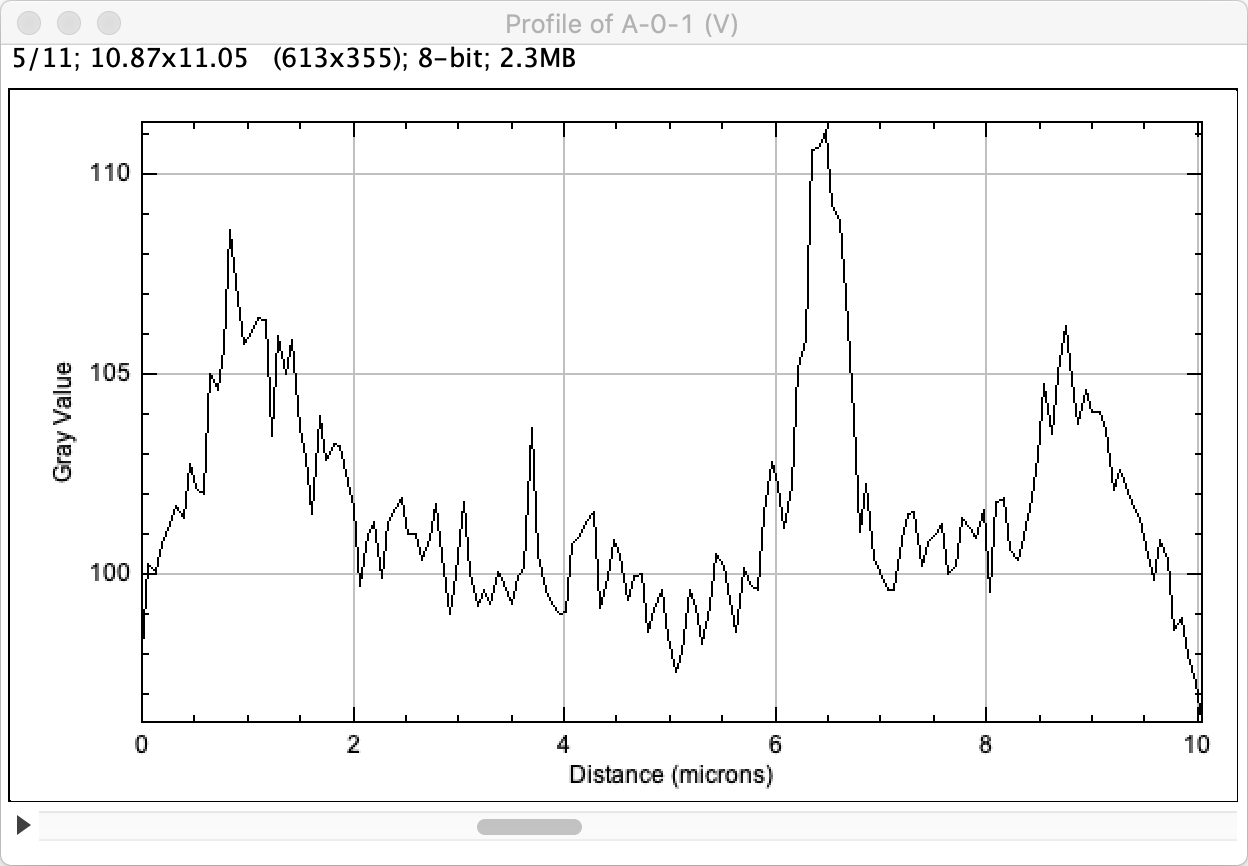
\includegraphics[width=\textwidth]{images/ui-plot-profiles.png}
    \caption{\centering Stos profili intensywności pod łamaną opisującą komórkę na kanale z~fluorescencją.}
  \end{subfigure}
  \hfill

  \par\bigskip

  \begin{subfigure}[t]{.45\textwidth}
    \centering
    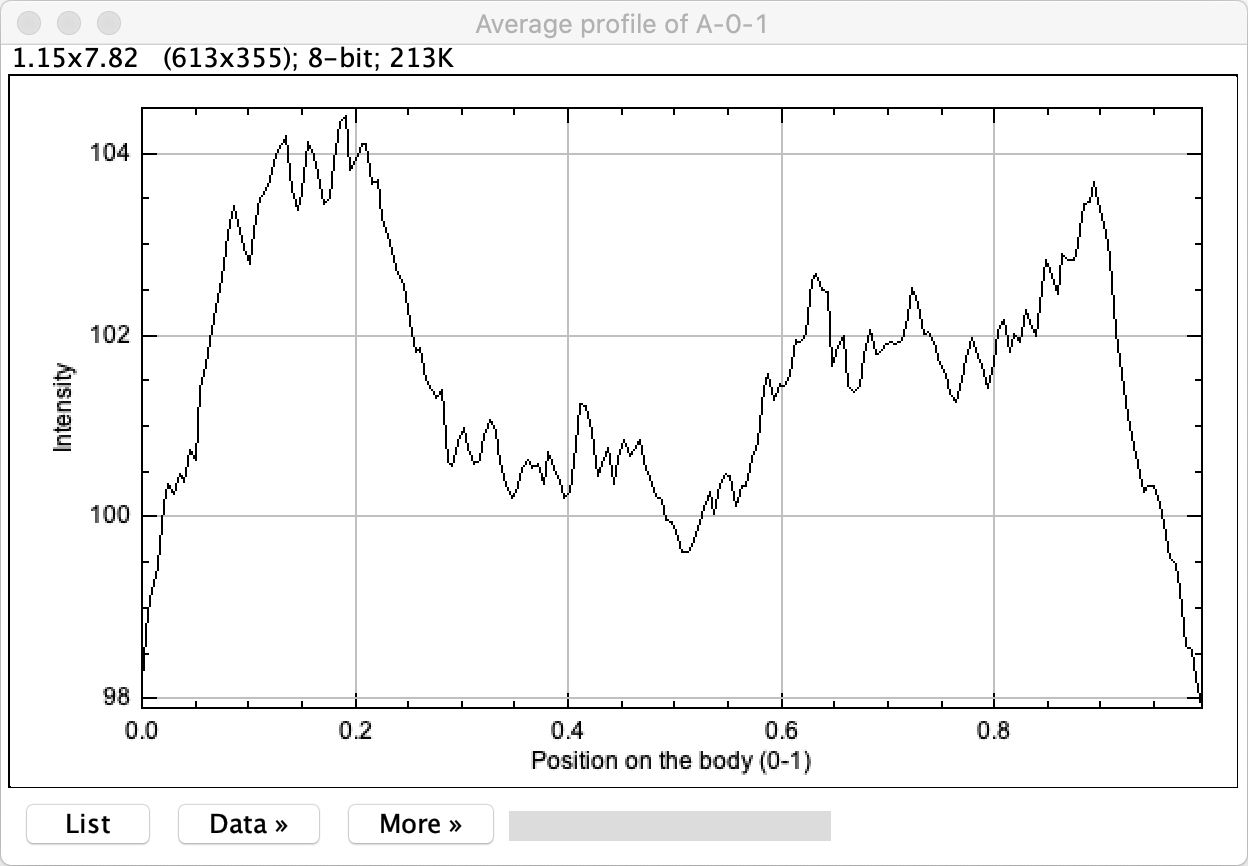
\includegraphics[width=\textwidth]{images/ui-plot-avg-profile.png}
    \caption{\centering Średni profil intensywności pod łamaną opisującą komórkę na kanale z~fluorescencją.}
  \end{subfigure}
  \hfill
  \begin{subfigure}[t]{.45\textwidth}
    \centering
    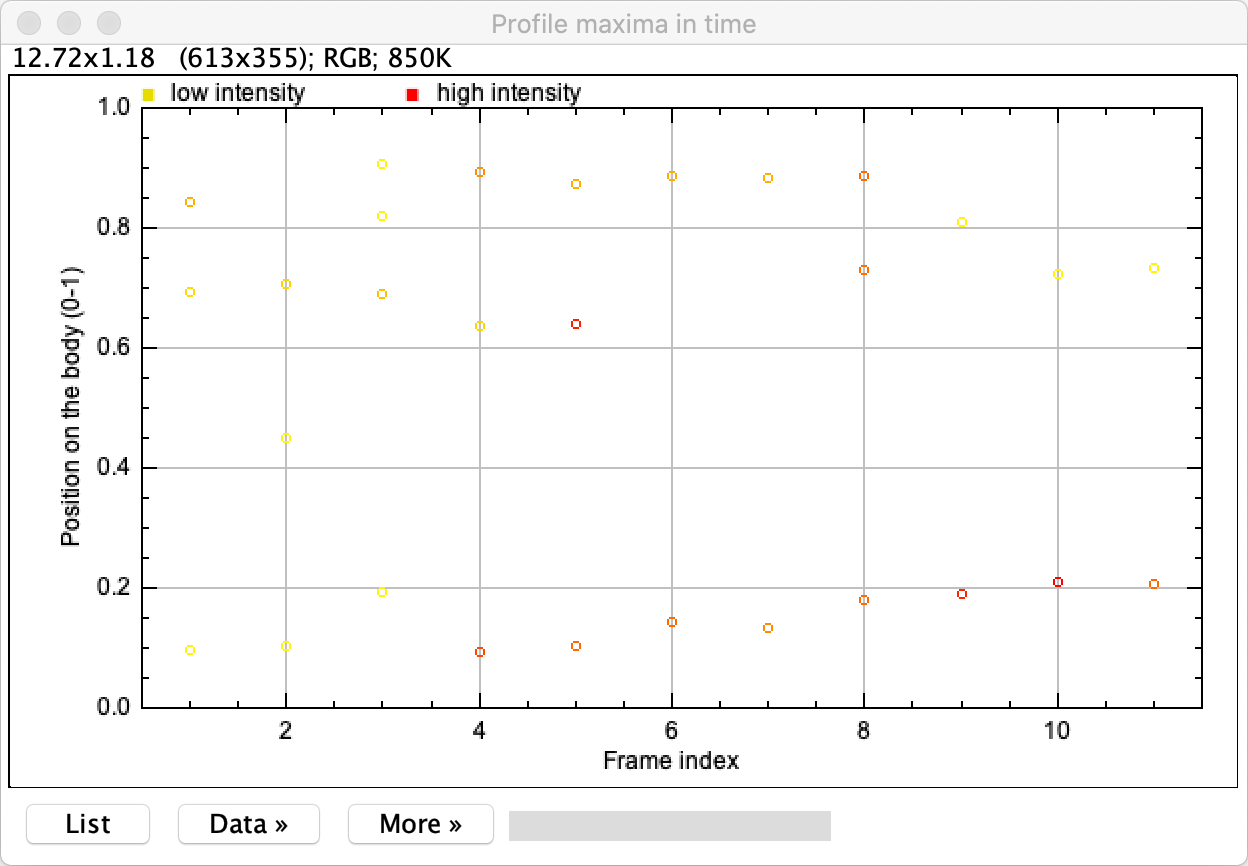
\includegraphics[width=\textwidth]{images/ui-plot-picks.png}
    \caption{\centering Umiejscowienie ,,skupisk'' na kanale z~fluorescencją w~czasie.}
  \end{subfigure}
  \hfill

  \caption{Różne rodzaje wykresów.}
  \label{fig:ui-plots}
\end{figure}

W celu analizy profili i~długości komórek poza programem można, za pomocą kolejnych przycisków, wyeksportować dane pojedynczej lub wszystkich komórek do formatu \texttt{CSV} (ang. comma-separated values).


\subsection{Manualna modyfikacja komórek}
\label{sec:user-manual-modifications}

W celu manualnej modyfikacji komórki należy wybrać ją w~oknie \texttt{ROI Manager} (rysunek \ref{fig:ui-roi-manager}), które otwierane jest automatycznie podczas pracy z~komórkami.
Komórka na obrazie będzie wyświetlona w~postaci standardowego zaznaczenia wykonanego narzędziem do zaznaczania linii łamanej (ang. Segmented Line Selection Tool)\cite{imagej:segmented-line}.
Przesuwanie, usuwanie lub dodawanie wierzchołków takiego zaznaczenia zapisywane jest także dla komórki.
Komórki usunięte z~listy okna \texttt{ROI Manager} zostaną usunięte również z~kolekcji wraz z~zaznaczeniami w~kolejnych klatkach, jak i~komórkami pochodnymi.
Kolekcja zaznaczeń dla poprzednich klatek pozostanie bez zmian.

\begin{figure}
  \centering
  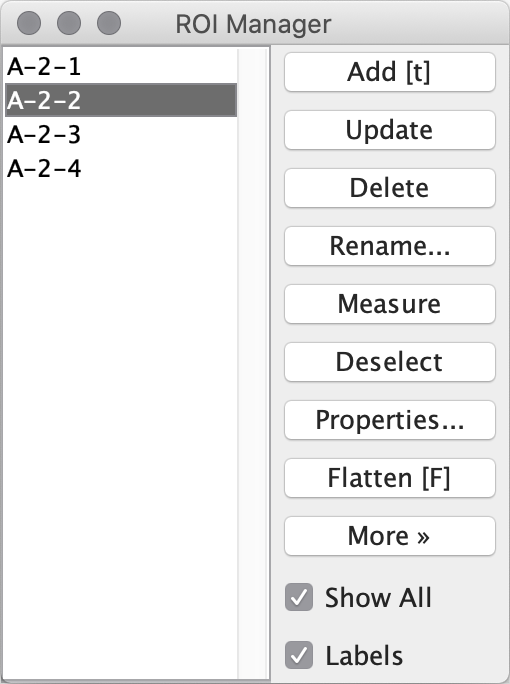
\includegraphics[width=0.3\textwidth]{images/ui-roi-manager.png}
  \caption{Okno \texttt{ROI Manager} pozwalające na wybór komórki.}
  \label{fig:ui-roi-manager}
\end{figure}

Ponadto okno pluginu wyposażone jest w~dwa dodatkowe narzędzia mające ułatwić manualną edycję komórek. Narzędzia można włączyć za pomocą przycisków widocznych w~lewym dolnym rogu okna pluginu.

Tryb rozcinania komórek można aktywować za pomocą przycisku z~ikoną w~kształcie nożyczek (\raisebox{-0.1em}{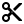
\includegraphics[width=0.9em]{images/tool-cut.png}}).
Służy on do ręcznego oznaczania punktów podziału komórek. Po jego uruchomieniu użytkownik może ,,przeciąć'' komórkę rysując symboliczną linię na obrazie.
Przecięta komórka zostanie podzielona na dwie komórki, które zostaną dodane do kolekcji jako kolejne pokolenia (,,dzieci'') komórki sprzed podziału (jeśli przecinana komórka występuje w~poprzedniej klatce).
Ze względu na specyfikę cyklu komórkowego, nie jest możliwe doprowadzenie do stanu w~którym jedna komórka dzieli się na więcej niż dwie części.
Należy pamiętać, że rozcięcie komórki, która została oznaczona w~późniejszych klatkach, wiąże się z~utratą jej zaznaczeń w~tych klatkach oraz usunięciem kolejnych pokoleń pochodzących od tej komórki.

Drugim dodatkowym narzędziem jest tryb skracania końcówek, uruchamiany za pomocą przycisku z~ikoną w~kształcie gumki do mazania (\raisebox{-0.1em}{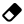
\includegraphics[width=0.9em]{images/tool-erase.png}}).
Działa on podobnie do narzędzia ,,gumki'' obecnego w~popularnych programach graficznych. Za jego pomocą nie można podzielić komórki, ale można ją skrócić lub całkowicie usunąć.
Jeśli komórka zostanie ,,wymazana'' w~całości to, analogicznie jak przy usuwaniu komórki z~poziomu okna \texttt{ROI Manager}, usunięte zostaną również zaznaczenia w~kolejnych klatkach oraz kolejne pokolenia pochodzące od tej komórki.

\subsection{Nazewnictwo komórek oraz ich orientacja}
\label{sec:cell-naming}

Aby ułatwić identyfikację komórek, przyjąłem stałą konwencję ich nazewnictwa.
Nazwa składa się z~trzech członów: identyfikatora komórki źródłowej, indeksu pokolenia oraz indeksu w~ramach pokolenia.
Komórkom źródłowym (nie mającym rodzica) zostaje przydzielony unikalny identyfikator w~postaci wielkiej litery alfabetu.
Indeks pokolenia jak i~indeks w~ramach pokolenia wynikają z~natury kolekcji komórek.
Każda komórka dzieli się w~pewnym momencie na dwie nowe komórki (dzieci) nowego pokolenia.
,,Drzewo genealogiczne'' komórek będzie w~takim przypadku drzewem binarnym, a~indeksy pokolenia i~w ramach pokolenia będą odpowiednio odległością od korzenia i~liczbą porządkową w~ramach tego samego indeksu pokolenia.
Przykładowe drzewo pokrewieństwa opisane nazwami komórek przedstawia rysunek \ref{fig:tree-naming}.


\begin{figure}[h]
  \Tree
    [.\texttt{A-0-1}
      [.\texttt{A-1-1}
        [.\texttt{A-2-1}
          {\ldots}
          {\ldots}
        ]
        [.\texttt{A-2-2}
          {\ldots}
          {\ldots}
        ]
      ]
      [.\texttt{A-1-2}
        [.\texttt{A-2-3}
          {\ldots}
          {\ldots}
        ]
        [.\texttt{A-2-4}
          {\ldots}
          {\ldots}
        ]
      ]
    ]
  \caption{Drzewo genealogiczne opisane zgodnie z~konwencją nazewnictwa.}
  \label{fig:tree-naming}
\end{figure}

Dzięki tak skonstruowanej konwencji nazewnictwa można łatwo zidentyfikować pochodzenie komórki, a~także stopień pokrewieństwa z~innymi komórkami.

W celu zapewnienia spójności analizowanych na końcu danych, ustaliłem również stałą orientację komórek.
Aby móc rozróżnić końcówki komórek, wystarczy zaznaczyć opcję \texttt{show endpoints} w~dolnej części okna pluginu.
Kolorem czerwonym oznaczone zostaną końcówki powstałe w~wyniku podziału komórki, a~zielonym te które były wcześniej końcówkami komórki rodzica (rysunek \ref{fig:ui-show-endpoints}). W~przypadku komórki źródłowej końcówki oznaczone są losowo.

\begin{figure}
  \centering
  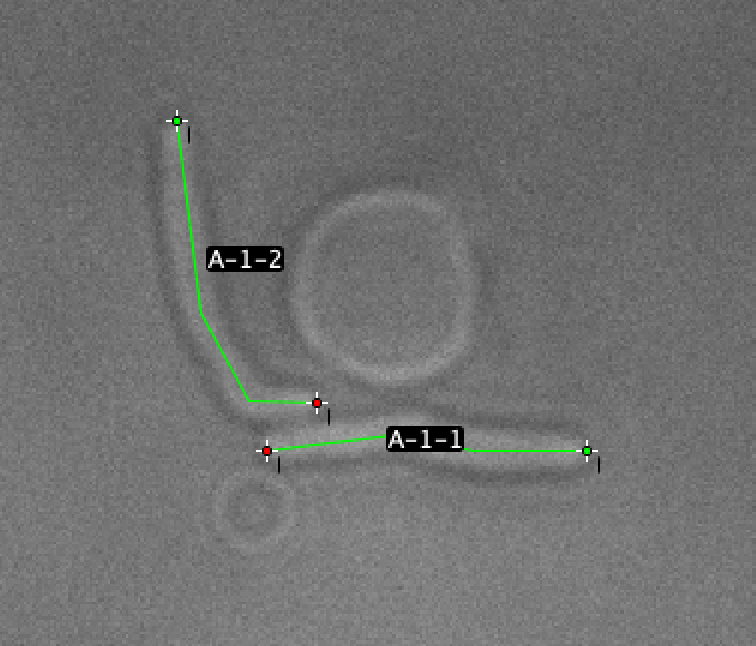
\includegraphics[width=0.3\textwidth]{images/ui-show-endpoints.png}
  \caption{Komórki wraz ze znacznikami identyfikującymi końcówki.}
  \label{fig:ui-show-endpoints}
\end{figure}

\subsection{Importowanie i eksportowanie komórek}

Manualne oznaczanie i~poprawianie komórek może być czasochłonne i~nie zawsze można zakończyć pracę w~ciągu jednej sesji.
Aby nie utracić efektów swojej pracy, użytkownik może wyeksportować oznaczone komórki za pomocą menu \texttt{Mycobacterium > Export cells}.
Stworzony w~ten sposób plik \texttt{XML} jest wynikiem serializacji kolekcji komórek.
Podczas kolejnej sesji, po otwarciu tego samego nagrania, zapisane komórki można wczytać korzystając z~menu \texttt{Mycobacterium > Import cells}.

\section{Dokumentacja techniczna}

\subsection{Struktura projektu}

Główna struktura plików projektu podzielona jest zgodnie z~konwencją zaproponowaną przez zespół Apache Maven\cite{docs:maven-project-layout}. Główne foldery to:
\begin{itemize}
  \item \texttt{src/main/java} -- kod źródłowy aplikacji
  \item \texttt{src/main/resources} -- zasoby aplikacji np. obrazki
  \item \texttt{src/test/java} -- kod źródłowy testów automatycznych.
\end{itemize}

Kod źródłowy aplikacji podzielony jest na kilka folderów, ze względu na aspekt którego dotyczy:

\begin{itemize}
  \item \texttt{cells} -- kod zawierający logikę dotyczącą domeny pracy, m.in. kod pluginu, interfejsy poszczególnych kroków, główne algorytmy itp.; wewnątrz wydzielono dodatkowo foldery:
  \begin{itemize}
    \item[$\circ$] \texttt{serialization} -- kod dotyczący importu i~eksportu komórek
    \item[$\circ$] \texttt{skeleton} -- implementacja króków detekcji i~śledzenia komórek opisana w~tej pracy (oparta na szkieletyzacji)
    \item[$\circ$] \texttt{measurements} -- implementacja etapu analizy danych
  \end{itemize}
  \item \texttt{graph} -- implementacja grafu
  \item \texttt{gui} -- implementacje generycznych okien i~komponentów interfejsu
  \item \texttt{imagej} -- klasy ułatwiające prace i~komunikację z~programem--hostem ImageJ
  \item \texttt{util} -- inne pomocnicze klasy
  \item \texttt{vendor} -- publicznie dostępne wtyczki do programu ImageJ lub opakowania ułatwiające korzystanie z~zależności zadeklarowanych w~\texttt{pom.xml}.
\end{itemize}

\subsubsection{Konwencja nazewnictwa}

Nazwy interfejsów rozpoczynają się od wielkiej litery ,,\texttt{I}'' np. \texttt{ICellsPluginStep}, natomiast nazwy klas abstrakcyjnych zaczynają się od prefiksu ,,\texttt{Abstract}'' np. \texttt{AbstractCellCollection}.

\subsection{Główne struktury danych}

\subsubsection{\texttt{AbstractCellCollection}}

Ta abstrakcyjna klasa służy do opisywania drzewiastej struktury komórek. Dziedziczą po niej dwie klasy: \texttt{CellCollection} oraz \texttt{Cell}.
Ta pierwsza służy do przechowywania kolekcji komórek reprezentowanych przez klasę \texttt{Cell}.
Druga natomiast oprócz reprezentowania komórki, może zawierać także referencje do dwóch komórek potomnych, tworząc w~ten sposób binarne ,,drzewo genealogiczne'' komórki.

Klasa deklaruje m.in. metody dodawania i~usuwania komórek z~kolekcji, ale także metody do wydobywania wszystkich komórek ,,żyjących'' w~danej klatce nagrania.

Klasy dziedziczące po \texttt{AbstractCellCollection} muszą być serializowalne.
Własność ta jest wykorzystywana podczas importowania i~eksportowania komórek do pliku \texttt{XML}.

\subsubsection{\texttt{Cell}}

Jest to klasa opisująca komórkę i~cały jej cykl życia -- od pojawienia się, do momentu podziału na dwie nowe komórki (może zawierać także referencje do tych komórek potomnych).
Obiekt tej klasy zawiera informacje o~każdej klatce w~której występuje komórka w~postaci referencji do instancji \texttt{AbstractCellFrame}.
Pozwala też określić i~odczytać poszczególne części nazwy komórki takie jak identyfikator komórki źródłowej, indeks pokolenia czy indeks w~ramach pokolenia (\ref{sec:cell-naming}).

Poza wyżej wymienionymi oraz dziedziczonymi po klasie \texttt{AbstractCellCollection} funkcjonalnościami, obiekt tej klasy zawiera również metody potrzebne do uzyskania reprezentacji komórki w~postaci standardowego zaznaczenia w~programie ImageJ.

\subsubsection{\texttt{AbstractCellFrame}}

Klasa ta deklaruje metody służące do uzyskania zaznaczenia pojedynczej komórki w~konkretnej klatce nagrania, a~także do modyfikacji tego zaznaczenia.

Na potrzeby tej pracy powstała jej implementacja \texttt{PolylineCellFrame}, która reprezentuje zaznaczenie komórki w~postaci linii łamanej.

\subsubsection{\texttt{Graph}, \texttt{Edge}, \texttt{Vertex}, \texttt{Point}}

Klasy te składają się na implementację grafu, który zawiera dodatkowe informacje o~punktach reprezentowanych przez krawędzie i~wierzchołki.

\subsection{Architektura umożliwiająca dalszy rozwój}
\label{sec:architecture}

Główną klasą projektu jest \texttt{CellsPlugin}, która instancjonowana jest przez program ImageJ po otwarciu wtyczki z~poziomu menu \texttt{Mycobacterium > Cell Detector}.
Podczas uruchomienia tworzona jest kopia aktualnie otwartego stosu obrazów, która wyświetlona zostaje w~specjalnym oknie pluginu (jego opis znajduje się w~rozdziale \ref{sec:user-manual}), a~także utworzona zostaje pusta kolekcja komórek.

Podczas inicjalizacji uruchomiony zostaje również nasłuch na różnego rodzaju zdarzenia programu--hosta ImageJ m.in. na:
\begin{itemize}
  \item zmiany podglądu obrazu -- umożliwia to wyświetlenie odpowiednich komórek dla aktualnie oglądanej klatki
  \item zmiany zaznaczeń na obrazie -- dzięki temu zmiany mogą być zapisywane dla komórek opisywanych przez zmodyfikowane zaznaczenia
  \item zmianę aktywnego narzędzia -- może mieć wpływ na zachowanie wybranego narzędzia specjalnego (\ref{sec:user-manual-modifications})
  \item zmiany na liście okna \texttt{Roi Manager} -- umożliwia to usuwanie komórek z~poziomu tego okna.
\end{itemize}

Każdy z~trzech etapów pluginu (wstępna detekcja, śledzenie komórek i~analiza danych) jest obiektem klasy implementującej interfejs \texttt{ICellsPluginStep}.
Interfejs ten deklaruje zaledwie trzy publiczne metody:

\begin{itemize}

\item \texttt{JComponent init(ImagePlus imp, CellCollection cells)}

Metoda ta wywoływana jest podczas inicjalizacji danego kroku np. przy starcie pluginu (dla kroku wstępnej detekcji) lub przy wciśnięciu przycisku \texttt{next} (dla kolejnego kroku).
Argumentami są obraz źródłowy (nagranie) oraz referencje do kolekcji komórek.
Metoda odpowiedzialna jest również za stworzenie i~zwrócenie komponentu interfejsu danego kroku, który zostanie automatycznie umieszczony w~odpowiednim miejscu okna wtyczki.

\item \texttt{void imageUpdated()}

Ta metoda służy do nasłuchiwania na zmiany obrazu i~wyświetlanych komórek.
Uruchamiana jest przez plugin dla aktywnego kroku po każdej aktualizacji podglądu obrazu i~komórek na nim wyświetlonych.

\item \texttt{void cleanup()}

Metoda ta wywoływana jest podczas zmiany aktualnego kroku lub przy zamknięciu pluginu.

\end{itemize}

Instancja klasy implementującej interfejs \texttt{ICellsPluginStep} tworzona jest za pomocą metody \texttt{Class.newInstance}.
Do jej stworzenia użyty zostanie konstruktor niewymagający podania argumentów.

Dzięki tak zaprojektowanemu systemowi każdy z~etapów programu jest niezależny i~może zostać z~łatwością wymieniony na inną implementację tego interfejsu.
Klasy które mają zostać użyte są zadeklarowane jako statyczne stałe \linebreak
\texttt{CellsPlugin.StepDetectorClass}, \texttt{CellsPlugin.StepLifeTrackerClass} oraz \linebreak
\texttt{CellsPlugin.StepMeasurementsClass}.

W aktualnej wersji pluginu implementacjami poszczególnych kroków są klasy \texttt{SkeletonCellDetector}, \texttt{SkeletonCellLifeTracker} oraz \texttt{StepMeasurements}.\linebreak
Przykładowo chcąc użyć klasy \texttt{ExampleLifeTracker} jako innej implementacji kroku śledzenia komórek, należy upewnić się że implementuje ona interfejs opisany powyżej, a~następnie zmienić wartość stałej \texttt{CellsPlugin.StepLifeTrackerClass} na \texttt{ExampleLifeTracker.class}.

Kod pluginu zawiera wszystkie główne struktury danych (lub ich abstrakcyjne wersje) i~dzięki temu jest zupełnie niezależny od implementacji poszczególnych kroków -- komunikuje się z~nimi jedynie za pomocą opisanych wyżej interfejsów.
Funkcjonalności niezależne od implementacji poszczególnych etapów takie jak wyświetlanie, usuwanie i~ręczna modyfikacja komórek, a~także ich eksportowanie i~importowanie, bazują wyłącznie na metodach deklarowanych przez odpowiednie interfejsy lub klasy abstrakcyjne.

\subsubsection{Przykładowa implementacja pojedynczego etapu pluginu}

Poniższy fragment kodu przedstawia przykładową implementację kroku śledzenia komórek.
Jest to uproszczona implementacja wyświetlająca jedynie przycisk \texttt{duplicate}, który umożliwia skopiowanie aktualnych zaznaczeń do kolejnej klatki.

\par\bigskip

\begin{lstlisting}
public class ExampleLifeTracker implements ICellsPluginStep {
  ImagePlus imp;
  CellCollection cellCollection;

  @Override
  public JComponent init(ImagePlus imp, CellCollection cellCollection) {
    this.imp = imp;
    this.cellCollection = cellCollection;

    JPanel component = new JPanel();
    component.setLayout(new BoxLayout(component, BoxLayout.Y_AXIS));
    component.add(new RunnableButton("duplicate", this::onDuplicateClick));
    return component;
  }

  @Override
  public void imageUpdated() {
    // ignore
  }

  @Override
  public void cleanup() {
    // ignore
  }

  void onDuplicateClick() {
    int currentFrameIndex = imp.getT();
    // get list of cells visible at current frame
    List<Cell> cells = cellCollection.getCells(currentFrameIndex);
    int nextFrameIndex = currentFrameIndex + 1;
    if (cells.size() < 1 || nextFrameIndex > imp.getNFrames()) {
      return;
    }
    // clear previous selections for next frames
    cells.forEach(cell -> cell.clearFuture(nextFrameIndex));
    cells.forEach(cell -> {
      // clone current selection
      AbstractCellFrame duplicate = cell.getFrame(currentFrameIndex).clone();
      // set selection for next frame to cloned value
      cell.setFrame(nextFrameIndex, duplicate);
    });
    // show next frame
    imp.setT(nextFrameIndex);
    // update image and cells preview
    imp.updateAndDraw();
  }
}
\end{lstlisting}

Podczas inicjalizacji zapisywane są referencje do obrazu wejściowego \texttt{imp} oraz do kolekcji komórek \texttt{cellCollection}, a~następnie tworzony jest komponent zawierający jeden przycisk.
Wciśnięcie przycisku \texttt{duplicate} powoduje wywołanie metody \texttt{onDuplicateClick}, która duplikuje zaznaczenia widoczne w~aktualnej klatce do kolejnej klatki.
Jeśli w~aktualnej klatce nie ma żadnych zaznaczeń lub jest to ostatnia klatka nagrania, metoda nie powoduje żadnego efektu.
Zwrócony przez metodę \texttt{init} komponent zostanie automatycznie umieszczony w~oknie pluginu.

Załóżmy że chcemy jeszcze dodatkowo zmienić podgląd obrazu, tak aby zamiast oryginalnego obrazu użytkownik widział mapę indeksów kształtu.
Można to zrobić nakładając dodatkową warstwę \texttt{Overlay} na podgląd obrazu.

\par\bigskip

\begin{lstlisting}
public class ExampleLifeTracker implements ICellsPluginStep {

  // ...

  @Override
  public void imageUpdated() {
    ImagePlus frame = HyperstackHelper.extractFrame(imp);
    ImagePlus shapeIndexMap = ShapeIndexMap.getShapeIndexMap(frame, 4.0);
    ImageRoi roi = new ImageRoi(0, 0, shapeIndexMap.getProcessor());
    Overlay overlay = new Overlay();
    overlay.add(roi);
    imp.setOverlay(overlay);
  }

  @Override
  public void cleanup() {
    imp.setOverlay(null);
  }

  // ...

}
\end{lstlisting}

Metoda \texttt{imageUpdated} zostanie wywołana przy każdej aktualizacji oryginalnego obrazu np. gdy zmieni się wyświetlana klatka lub kanał.
Po przejściu do kolejnego etapu pluginu zostanie wywołana metoda \texttt{cleanup}, która w~powyższej wersji usunie dodatkową warstwę przywracając tym samym podgląd do oryginalnej wersji.

Analogicznego mechanizmu używają aktualne implementacje kroku detekcji oraz śledzenia komórek do wyświetlenia podglądu mapy indeksów kształtu lub szkieletu (\texttt{advanced settings}).

\subsection{Wykorzystywane API ImageJ}

ImageJ jest częścią większego ekosystemu SciJava.
Projekty tworzone w~ramach tego ekosystemu są wytwarzane jako otwarte oprogramowanie z~publicznie dostępnym kodem.
ImageJ jest nie tylko programem, ale rozszerzalną platformą zbudowaną na architekturze opartej o~mechanizm pluginów.
Stanowi to jeden z~największych atutów tej platformy\cite{imagej:philosophy}.

Plugin został napisany przy wykorzystaniu nowszego API ImageJ2, jednak korzysta również z~warstwy zapewniającej kompatybilność z~ImageJ 1.x.
Spowodowane jest to głównie brakiem dobrej dokumentacji istotnych funkcjonalności dla nowszej wersji API, dostępnej w~trakcie implementacji projektu.

W moim programie zdecydowałem się użyć natywnych dla ImageJ narzędzi do tworzenia zaznaczeń (ROIs, ang. regions of interest), w~celu wyświetlania i~modyfikacji komórek.
Dzięki temu nie musiałem tworzyć od nowa mechanizmów służących do wyświetlania wielu linii łamanych na obrazie, a~także do ich modyfikacji.
Również narzędzia do przecinania i~skracania końcówek są tak naprawdę nakładką na standardowe narzędzia do zaznaczania linii i~zaznaczania za pomocą pędzla.

\subsection{Brakujące lub niespójne API ImageJ}

W tak dużym otwartym oprogramowaniu tworzonym przez dużą społeczność nie sposób uniknąć niespójności czy obsłużyć wszystkie warunki brzegowe.
Implementując niektóre funkcjonalności zdecydowałem się użyć standardowych narzędzi ImageJ, w~celu nieco innym niż ich oryginalne przeznaczenie.
Ze względu na to, potrzebowałem niskopoziomowego dostępu do różnych mechanizmów za tym stojących, aby wstrzyknąć tam własną warstwę pośredniczącą.
Twórcy ImageJ, mając na uwadze potrzebę rozszerzalności, wyposażyli tę platformę w~szereg narzędzi mających w~tym pomóc.
Mimo wszystko kilka elementów systemu okazało się działać nie do końca zgodnie z~intuicją i~wymagało niezbyt eleganckiego rozszerzenia.

\subsubsection{Nasłuchiwanie na zdarzenia modyfikacji ROI}

Chcąc rejestrować wydarzenia na temat modyfikacji wyświetlanych aktualnie zaznaczeń, należy zaimplementować interfejs \texttt{RoiListener}, a~następnie tę implementację zarejestrować przekazując ją do statycznej metody \texttt{Roi.addRoiListener}.
Słuchacz będzie otrzymywać zgłoszenia na temat różnych wydarzeń związanych z~zaznaczeniami m.in. na temat ich utworzenia, przesunięcia, modyfikacji, rozszerzenia, ukończenia czy usunięcia.
W moim programie nasłuchiwanie na te wydarzenia odgrywa kluczową rolę.
Zdiagnozowałem kilka miejsc, w~których moim zdaniem system notyfikacji działa niezgodnie z~intuicją:
\begin{itemize}
  \item Tworzenie zaznaczenia w~kształcie linii polega na oznaczeniu kursorem myszy punktu początkowego, wciśnięciu głównego klawisza myszy, przeciągnięciu kursora do miejsca docelowego, a~następnie zwolnieniu klawisza myszy. Konstruując zaznaczenie w~kształcie linii, słuchacz dostaje informacje na temat wydarzenia związanego z~modyfikacją, natomiast po zwolnieniu przycisku myszy nie jest zgłaszane żadne wydarzenie. Intuicja podpowiada mi, że powinno zostać zgłoszone wydarzenie związane z~ukończeniem konstrukcji zaznaczenia.
  \item Analogiczny problem występuje w~przypadku zaznaczania za pomocą pędzla. Tutaj proces zaznaczania podobny jest do ,,malowania'' narzędziem pędzla w~popularnych programach graficznych. Również w~tym przypadku po zwolnieniu przycisku myszy nie jest zgłaszane żadne wydarzenie.
  \item Zaznaczenie w~postaci lini łamanej może być modyfikowane na różne sposoby. Można przeciągać całą linię łamaną lub modyfikować jej wierzchołki poprzez ich przeciąganie, usuwanie lub dodawanie. W~przypadku przesunięć całego zaznaczenia jak i~w przypadku zmiany pozycji poszczególnych wierzchołków zgłaszane są poprawne wydarzenia (odpowiednio o~przesunięciu i~modyfikacji). Jednak w~przypadku usuwania i~dodawania wierzchołków żadne wydarzenie nie jest zgłaszane.
\end{itemize}

W celu rozwiązania pierwszych dwóch problemów postanowiłem stworzyć własną warstwę aplikacji (\texttt{RoiObserver}) odpowiedzialną za obserwowanie zmian zaznaczeń.
Nasłuchuje ona na zmiany zaznaczeń poprzez interfejs \texttt{RoiListener}, ale także nasłuchuje na zdarzenia związane z~interakcją między kursorem myszy, a~otwartymi oknami obrazów.
Podczas konstrukcji problematycznych zaznaczeń zapisywane są ich referencje, aby następnie po otrzymaniu informacji o~zwolnieniu przycisku myszy wyemitować brakujące wydarzenie.

Trzeci problem został rozwiązany poprzez utworzenie i~korzystanie z~nowej klasy rozszerzającej zaznaczenie w~kształcie lini łamanej.
Nadpisuje ona tylko jedną metodę \texttt{PolygonRoi.mouseDownInHandle}, która używana jest do tworzenia i~usuwania dodatkowych wierzchołków -- odbywa się to przez kliknięcie kursorem myszy w~wierzchołek, mając przy tym wciśnięty klawisz \texttt{alt} lub \texttt{control}.
Nowa wersja metody wywołuje oryginalną, zachowując przy tym pierwotny sposób działania, a~następnie zgłasza wydarzenie związane z~modyfikacją.

\subsubsection{Usuwanie ROI z poziomu okna \texttt{ROI Manager}}

Najbardziej naturalnym sposobem na usunięcie komórki (np. w~przypadku gdy została niepoprawnie podzielona), wydaje się zaznaczenie jej na liście okna \texttt{ROI Manager} i~wciśnięcie przycisku \texttt{Delete} na klawiaturze lub z~poziomu interfejsu.
Bez specjalnej obsługi takiego zachowania, zaznaczenie komórki zniknęłoby, mimo że komórka wciąż pozostawałaby w~kolekcji i~po odświeżeniu podglądu znów pojawiłaby się na ekranie.
Takie zachowanie byłoby nieintuicyjne z~perspektywy użytkownika.
Postanowiłem więc stworzyć odpowiednią obsługę takiej sytuacji.
Okazało się jednak, że nie istnieje żadne narzędzie pozwalające otrzymywać powiadomienia na temat usuniętego z~poziomu tego okna zaznaczenia.

Problem ten rozwiązałem poprzez odnalezienie referencji do jednego z~komponentów okna \texttt{ROI Manager}, służącego do wyświetlania listy komórek.
Pozwala on na nasłuchiwanie na zmianę zawartości, w~szczególności usunięcie jednego lub wielu elementów.
Po otrzymaniu takiego powiadomienia, stan listy porównywany jest z~kolekcją komórek, które powinny aktualnie być wyświetlane -- te których brakuje na liście usuwane są również z~kolekcji.
Rozwiązanie to nie jest wyjątkowo stabilne, ponieważ dokonuje konwersji typów bazując na strukturze komponentów z~jakich składa się okno \texttt{ROI Manager}.
Wymaga również każdorazowej ingerencji w~to okno podczas jego uruchamiania.


%%%%%%%%%%%%%%%%%%%%%%%%%%%%%%%%%%%%%%%%%%%%%%%%%%%%%%%%%%%%%%%%%%%%%%%%%%%%%%%%%%%%%%%%%%%

\chapter{Zakończenie}

%%%%%%%%%%%%%%%%%%%%%%%%%%%%%%%%%%%%%%%%%%%%%%%%%%%%%%%%%%%%%%%%%%%%%%%%%%%%%%%%%%%%%%%%%%%


\section{Podsumowanie}

Efektem niniejszej pracy jest narzędzie, mające usprawnić proces pozyskiwania danych na temat cyklu komórkowego bakterii z~gatunku \emph{Mycobacterium smegmatis}.
Narzędzie to zostało stworzone jako plugin dla programu ImageJ, powszechnie używanego przez biologów, a~szczególnie przez mikrobiologów.
Wtyczka pozwala na oznaczanie komórek na kolejnych klatkach nagrania przedstawiającego cykl komórkowy \emph{M.~smegmatis}, tworząc w~ten sposób strukturę danych która w~późniejszych etapach służy do dokładnej analizy obrazów.
Oznaczanie komórek może odbywać się w~sposób w~pełni automatyczny, może być wspierane przez użytkownika poprzez wprowadzanie poprawek lub może odbywać się w~pełni manualnie.
Narzędzie zapewnia możliwość zapisu i~odczytu zaznaczeń z~pliku.
Wtyczka wyposażona jest dodatkowo w~narzędzia pomagające w~analizie cyklu komórkowego poprzez dokonywanie pomiarów, a~także tworzenie profili intensywności pod oznaczeniami komórek.
Dane można wyświetlić w~formie wykresów lub wyeksportować w~surowej formie w~celu analizy poza programem ImageJ (np. w~RStudio).

W pełni automatyczne oznaczanie i~śledzenie komórek nie zawsze jest możliwe.
Efekty tego podejścia są zadowalające tylko w~przypadku dobrych jakościowo nagrań.
Mimo to, nawet w~trybie w~pełni manualnym narzędzie może usprawnić pracę naukowców.
Plugin pozwala na usprawnienie podstawowych analiz danych mikroskopowych obejmujących m.in. pomiary długości komórek badanego szczepu bakteryjnego.
Tworzona w~pierwszych krokach struktura zawiera informacje o~rozwoju całej populacji komórek.
Może zostać zapisana i~wczytywana z~pliku, dzięki czemu użytkownik może podzielić swoją pracę w~czasie, wykorzystywać wielokrotnie raz utworzone zaznaczenia, a~także przesyłać je do innych użytkowników analizujących to samo nagranie.
Sam proces manualnego tworzenia zaznaczeń również został usprawniony poprzez możliwość skopiowania zaznaczeń z~poprzedniej klatki oraz stworzenie specjalnych narzędzi do wykonywania najczęściej powtarzających się czynności.

\section{Ograniczenia zastosowanych metod}

Przyjęta metoda automatycznego oznaczania i~śledzenia komórek nie jest wolna od ograniczeń.
Zakłada ona, że na obrazie binarnym, tworzonym na etapie szkieletyzacji, komórki (lub grupy komórek) są oddzielone od otoczenia.
Założenie to jest prawie zawsze spełnione w~miejscach, w~których w~okolicy grup komórek nie są widoczne żadne artefakty lub stałe elementy płytek po których poruszają się komórki.
Im lepsza była jakość nagrania (mniej szumów, mniej artefaktów, ostrzejsze krawędzie), tym lepiej radził sobie algorytm automatycznego śledzenia komórek.
Warto więc w~miarę możliwości zadbać o~wysoką jakość nagrania.

Przeciętne obrazy spod mikroskopu przedstawiające analizowane eksperymenty, zawierały wiele artefaktów.
Wady obrazów nakładające się z~komórkami często powodują błędne ich oznaczanie lub przedłużanie ich końcówek.
Zdarzało się również, że nagranie traciło ostrość w~niektórych momentach lub pole widzenia przesuwało się nieznacznie w~trakcie nagrania.
W pierwszym przypadku powodowało to całkowicie błędne oznaczenie komórek.
W drugim przypadku, odpowiednio duże przesunięcie również uniemożliwia poprawne odnalezienie lokalizacji komórek na podstawie oznaczenia z~poprzedniej klatki.

Jeśli krawędzie pomiędzy komórkami nie są wystarczająco ostre na nagraniu, to w~przypadku gdy pojawia się większa ilość komórek na raz, przestają one być oddzielone od siebie na obrazie binarnym.
W efekcie szkielet całego obrazu nie zawiera szkieletów poszczególnych komórek, co w~przyjętej metodzie uniemożliwia oznaczenie tych komórek.

\section{Dalszy rozwój}

Wymienione w~poprzednim rozdziale problemy zastosowanej metody automatycznego śledzenia komórek można spróbować rozwiązać korzystając ze znanych algorytmów z~dziedziny przetwarzania obrazów.
Aby zniwelować wpływ artefaktów na efekt końcowy, można by spróbować zastosować metody automatycznego ich usuwania na etapie wstępnego przetwarzania\cite{paper:removing-artifacts}.
Rozwiązaniem problemu związanego z~przesuwającym się w~trakcie nagrania polem widzenia, mogłoby być wyliczenie przesunięcia (translacji) poszczególnych klatek względem dowolnej klatki referencyjnej, na podstawie stałych elementów tła.
Takie dane mogłyby następnie zostać wykorzystane przy próbach określenia poprawnej lokalizacji komórek na podstawie poprzedniej klatki.

Tak jak wspomniałem w~rozdziale \ref{sec:detection-input}, w~niniejszej pracy nie zajmowałem się problemem określenia liczby i~lokalizacji poszczególnych komórek bez wcześniejszego udziału użytkownika.
Nawet w~trybie automatycznym użytkownik zobowiązany jest do zaznaczenia wszystkich komórek obecnych na pierwszej klatce nagrania.
Nie jest to duży wymóg, ponieważ komórek tych jest wtedy zazwyczaj niewiele.
Zaimplementowanie automatycznej detekcji komórek dla obrazów z~niewielką ich ilością mogłoby być jednak usprawnieniem aktualnego programu.

Podczas implementacji pluginu starałem się podejmować decyzje, które pozwoliłyby w~łatwy sposób rozwijać dalej ten projekt.
W rozdziale \ref{sec:architecture} opisałem w~jaki sposób można w~prosty sposób ,,wymienić'' dowolny etap pluginu, tj. lokalizację i~wstępną detekcję komórek, automatyczne śledzenie komórek, dokonywanie pomiarów i~wizualizacji na podstawie zaznaczeń.
Dzięki zastosowanemu podejściu, kod pluginu może zostać wykorzystany jako baza dla kolejnych prób znalezienia zupełnie nowej metody automatycznego oznaczania i~śledzenia komórek.




%%%%%%%%%%%%%%%%%%%%%%%%%%%%%%%%%%%%%%%%%%%%%%%%%%%%%%%%%%%%%%%%%%%%%%%%%%%%%%%%%%%%%%%%%%%

%%%%% BIBLIOGRAFIA

%%%%%%%%%%%%%%%%%%%%%%%%%%%%%%%%%%%%%%%%%%%%%%%%%%%%%%%%%%%%%%%%%%%%%%%%%%%%%%%%%%%%%%%%%%%


\begin{thebibliography}{1}

\bibitem{who-stats}
  World Health Organization,
  \emph{Tuberculosis},
  \url{https://www.who.int/news-room/fact-sheets/detail/tuberculosis},
  2020.

\bibitem{paper:watching-dna-replication}
  Damian Trojanowski, Marta Kołodziej, Joanna Hołówka, Rolf M{\"u}ller, Jolanta Zakrzewska-Czerwińska,
  \emph{Watching DNA Replication Inhibitors in Action: Exploiting Time-Lapse Microfluidic Microscopy as a~Tool for Target-Drug Interaction Studies in Mycobacterium},
  Antimicrobial Agents and Chemotherapy,
  American Society for Microbiology Journals,
  63(10),
  2019.
%  \url{https://aac.asm.org/content/63/10/e00739-19}

\bibitem{paper:protein-responsibility}
  Joanna Hołówka, Damian Trojanowski, Katarzyna Ginda, Bartosz Wojtaś, Bartłomiej Gielniewski, Dagmara Jakimowicz, Jolanta Zakrzewska-Czerwińska,
  \emph{HupB Is a~Bacterial Nucleoid-Associated Protein with an Indispensable Eukaryotic-Like Tail},
  mBio,
  American Society for Microbiology,
  8(6),
  2017.

\bibitem{paper:dic}
  Walter Lang,
  \emph{Nomarski differential interference-contrast microscopy},
  ZEISS Information,
  70:114–120,
  1968.

\bibitem{imagej:fiji}
  ImageJ User Guide,
  \emph{Fiji},
  \url{https://imagej.net/Fiji}.

\bibitem{app:rstudio}
  RStudio,
  \emph{RStudio IDE},
  \url{https://rstudio.com/products/rstudio}.

\bibitem{paper:detection-of-tb-with-ip}
  H. B. Rachna, M. S. Mallikarjuna Swamy,
  \emph{Detection of Tuberculosis Bacilli using Image Processing Techniques},
  International Journal of Soft Computing and Engineering,
  3:47-51,
  2013.

\bibitem{paper:ip-techniques-for-identifying-tb}
  P. Sadaphal, J. Rao, G. W. Comstock, M. F. Beg,
  \emph{Image processing techniques for identifying Mycobacterium tuberculosis in Ziehl-Neelsen stains},
  The international journal of tuberculosis and lung disease : the official journal of the International Union against Tuberculosis and Lung Disease,
  12(5):579–582,
  2008.

\bibitem{wiki:c-elegans}
  Wikipedia,
  \emph{Caenorhabditis elegans},
  \url{https://pl.wikipedia.org/wiki/Caenorhabditis_elegans}.

\bibitem{paper:worm-detection}
  Javier Fernández,
  \emph{Image Processing to Detect Worms},
  Uppsala Universitet,
  Uppsala,
  Sweden,
  2010.

\bibitem{paper:shape-index}
  Jan J~Koenderink, Andrea J~van Doorn,
  \emph{Surface shape and curvature scales},
  Image and Vision Computing,
  10:557--565,
  1992.

\bibitem{plugin:shape-index-map}
  Johannes Schindelin,
  \emph{Shape Index Map},
  2010,
  \url{https://imagej.net/Shape_Index_Map}.

\bibitem{algo:3d-thinning}
  Ta-Chih Lee, Rangasami L. Kashyap, Chong-Nam Chu,
  \emph{Building skeleton models via 3-D medial surface/axis thinning algorithms},
  Computer Vision, Graphics, and Image Processing,
  56(6):462--478,
  1994.

\bibitem{plugin:skeletonize-3d}
  Ignacio Arganda-Carreras,
  \emph{Skeletonize3D},
  2.1.1,
  2017,
  \url{https://imagej.net/Skeletonize3D}.

\bibitem{plugin:analyze-skeleton}
  Ignacio Arganda-Carreras,
  \emph{AnalyzeSkeleton},
  3.3.0,
  2018,
  \url{https://imagej.net/AnalyzeSkeleton}.

\bibitem{algo:ramer-douglas-peucker}
  Wikipedia,
  \emph{Ramer--Douglas--Peucker algorithm},
  \url{https://en.wikipedia.org/wiki/Ramer-Douglas-Peucker_algorithm}.

\bibitem{algo:ramer}
  Urs Ramer,
  \emph{An iterative procedure for the polygonal approximation of plane curves},
  Computer Graphics and Image Processing,
  1(3):224–256,
  1972.

\bibitem{algo:douglas-peucker}
  David Douglas, Thomas Peucker,
  \emph{Algorithms for the reduction of the number of points required to represent a~digitized line or its caricature},
  The Canadian Cartographer,
  10(2):112–122,
  1973.

\bibitem{imagej:segmented-line}
  ImageJ User Guide,
  \emph{Segmented Line Selection Tool},
  \url{https://imagej.nih.gov/ij/docs/guide/146-19.html#sub:Segmented-Line-Selection}.

\bibitem{docs:maven-project-layout}
  Apache Maven Project,
  \emph{Introduction to the Standard Directory Layout},
  \url{https://maven.apache.org/guides/introduction/introduction-to-the-standard-directory-layout.html}.

\bibitem{imagej:philosophy}
  ImageJ User Guide,
  \emph{Philosophy},
  \url{https://imagej.net/Philosophy}.

\bibitem{paper:removing-artifacts}
  Jinwei Gu, Ravi Ramamoorthi, Peter Belhumeur, Shree Nayar,
  \emph{Removing Image Artifacts Due to Dirty Camera Lenses and Thin Occluders},
  ACM Trans. Graph.,
  28(12),
  2009.

\end{thebibliography}

\end{document}
